\documentclass[12pt,a4paper,twoside,titlepage]{report}

\usepackage[english]{babel}
\usepackage[utf8]{inputenc}
\usepackage{fancyhdr}
\usepackage[paper=a4paper,margin=1in]{geometry}
\usepackage[chapter]{minted}
\usepackage{graphicx}

\graphicspath{{img/}}

\pagestyle{fancy}
\fancyhead[LE,RO]{}
\fancyhead[RE,LO]{\rightmark}
\fancyfoot[CE,CO]{}
\fancyfoot[LE,RO]{Page \thepage}
\renewcommand{\headrulewidth}{0.8pt}
\renewcommand{\footrulewidth}{0.8pt}

\usemintedstyle{borland}

\author{Ondřej~Hlavatý, Jan~Hrach, Jaroslav~Jindrák,\\Petr~Mánek, Michal~Staruch}
\title{HelenOS USB 3.x Stack}

\begin{document}

% The title page has its special margin.
\maketitle


% Use double-sided margins from now on.
\newgeometry{top=1in,bottom=1in,right=0.5in,left=1.5in}
\cleardoublepage

% Here come the macros.

% Use these semantically, we'll improve the style later

\newcommand{\app}[1]{\texttt{#1}}
\newcommand{\lib}[1]{\texttt{#1}}
\newcommand{\struct}[1]{\mintinline{c}{#1}}
\newcommand{\fnc}[1]{\mintinline{c}{#1}}

\newminted[bdsh]{shell}{autogobble,linenos,breaklines,frame=single,framesep=10pt}
\newminted[code]{c}{autogobble,linenos,breaklines,frame=single,framesep=10pt}




% Lists go in the front.
\tableofcontents
\newpage

\listoffigures
\newpage

\listoftables
\newpage

\listoflistings
\newpage

\cleardoublepage


% Here begins the actual content.
\chapter{Introduction}

\section{About HelenOS}
HelenOS is a microkernel operating system. Contrary to operating systems with
monolithic kernels, key operating system functionality (including device
drivers, filesystems and networking) is implemented in user-space processes (or
servers) that interact via message passing interface. The rationale of this
decision is that the failure of one component, e.g. a faulty driver, does not
result in the crash of the entire system. It also allows a more modular system
design.

HelenOS was started in 2004 as a software project at the Faculty of Mathematics
and Physics at Charles University and currently is being developed by students,
former students and staff of this university, among with a number of
contributors around the world. It has participated in Google Summer of Code
several times. HelenOS is used as a research operating system and as a platform
for bachelor and master theses and student software projects.

HelenOS supports several architectures (among them ia32, amd64, 32-bit ARM and
big endian MIPS) and is released under the BSD license.

\subsection{XHCI support in operating systems}

Extensible Host Controller Interface was first drafted in 2008 and the final
version of the specification was released in 2010. Since then, XHCI support
arrived in all mainstream operating systems like Windows, Linux, BSDs and Mac
OS X.

Regarding special-purpose, microkernel and research OSes, XHCI support is not
yet widespread.  Most notably, XHCI support is included in Google's
microkernel-based Fuchsia and in bare-metal iPXE.  Haiku Project is currently
developing XHCI driver for their OS.

\section{Drivers in HelenOS}
% TODO: Introduce DDF, terms like device, function, interfaces, add/remove/gone ops, ...

\section{Briefly about USB}
% TODO: Introduce reader to terms like speed, endpoint, transfer type, ...


\section{Existing USB Subsystem}

The support for USB was started by the HelUSB project defended in 2011. In that
time, the USB driver framework was designed, and delivered with few USB
drivers. From the Host Controller side, UHCI and OHCI were supported almost
completely. As for the device drivers, only a generic HID driver was provided
to demonstrate the functionality of the framework. Since the project was
delivered, the USB stack evolved a little and new drivers were implemented.

This document does not aim to replace the original documentation of HelUSB
project. As such, we will focus more on the things that changed since the
documentation was written, and they are pretty much not documented anywhere.
And by all means, information in this chapter is written with regard to the
state before our project was implemented. Thus, great part of the information
given in this section is already obsolete, but it's needed to assess the damage
we're personally responsible for.

The USB framework defines two classes of drivers -- the host controller drivers
and USB function drivers. For the first class, there is a library called
\lib{libusbhost} that aids in providing the unified interface of the host
controller to USB function drivers, and also implements common HC
functionality. There are four HC drivers at the moment:

\begin{itemize}
\item
	\textbf{VHC}, Virtual Host Controller. Implemented in the early phase of
	HelUSB project, served probably as a dummy backend to allow better work
	parallelization and debugging.

\item
	\textbf{UHCI}, Universal Host Controller Interface driver. The earliest
	interface supporting speeds of USB 1.0: Low- and Full-speed devices.
	Important for running HelenOS under QEMU, as it's the interface of the
	default HC QEMU emulates. Apart from isochronous transfers, the driver
	covers all functionality UHCI provides.

\item
	\textbf{OHCI}, Open Host Controller Interface driver. Somewhat complete,
	yet a bit simplified, especially in terms of transfer scheduling. Does not
	care about the polling interval, but schedules all interrupt transfers on
	every frame. Isochronous transfers not supported.

\item
	\textbf{EHCI}, Enhanced Host Controller Interface driver. Mostly a copy of
	OHCI driver, as it uses similar structures. Shall support USB 2 speeds, but
	the support is very limited -- the driver cannot use High-speed hubs to
	communicate with Full- and Low-speed devices, as the support for
	Transaction Translation is completely broken. Also, the bandwidth
	accounting is not implemented for High speed. Neither this controller
	supports isochronous transfers.
\end{itemize}

The HC driver is no longer split in half (as the project documentation states),
but all HC drivers emulate a virtual hub that is driven by a regular
\lib{usbhub} driver. The tree physical topology of USB is kept only inside the
HC driver, and is presented flat to the Device Driver Framework -- all USB
devices are child functions of the HC driver. They communicate with each other
through the DDF driver interface called \texttt{usb\_iface}, which contains all
methods various drivers use.

When the driver enumerates a USB function, it is usually taken care of by the
\lib{usbmid} driver. This driver scans the device descriptor for provided
interfaces, and create children functions for them. These functions are then
driven by class drivers. Notable exception being the \lib{usbhub} driver,
taking care of the device directly, as hubs are not allowed to have multiple
interfaces.

The USB function drivers are well supported by the \lib{libusbdev} library.
This library builds an abstraction layer above \lib{libdrv}, used by other
drivers directly, to better suit needs of USB devices. It does a complete
initialization of the USB device, including initiating a separate IPC
connection to the HC driver directly -- to avoid bouncing all operations in the
\lib{usbmid} driver. For this purpose, the \texttt{usb\_iface} contains two
methods: \fnc{get_my_iface} and \fnc{get_my_interface_handle}. The first one is
answered by the \lib{usbmid} driver with the number of interface driven, or
with a value of $-1$ by the HC driver if the driver serves the whole device.
The \fnc{get_my_interface_handle} call is recursive, until it reaches the HC
driver -- which answers it with devman handle of the USB device function. The
device driver then uses it to initiate connection to the HC driver, the same
way as the usbmid driver do.

Although this is sort-of hacky solution (the devman handle is supposed to be
private), it is currently the only one. Ideally, the drivers would use
a special method to let new connection forward to the HC driver, but for
complicated reasons, this does not work as expected. We discussed this with the
current HelenOS developers, and they confirmed us that the issue is still not
solved.

The \lib{usbhub} driver uses another four methods defined by the
\texttt{usb\_iface}. The interface methods \fnc{reserve_default_address} and
\fnc{release_default_address} ensure synchronization across multiple hubs
(possibly across multiple hub drivers), as the software must ensure that only one
device is listening on the default address at the same time. Then,
\fnc{device_enumerate} and \fnc{device_remove} announce that a device is
connected to (detached from) the hub, to be enumerated (removed) by the HC
driver. The interesting part is that the hub driver has no access to the
created device, as the logical topology presented to the DDF is flat.

All USB device drivers specify the endpoints they expect from the device in
a form of static description, which they pass to the \lib{libusbdev} library
during the driver initialization. Once a new device is added, the library
fetches the device descriptor and matches available endpoints against the
specification provided by the driver. Then the library creates \emph{pipes} --
an abstraction of endpoints based on their properties, not their exact numbers,
which are usually implementation defined. Pipes are then used by the driver
as, well, pipes to push data through and read data from.

The pipe creation process and their usage define the last four methods of which
the \texttt{usb\_iface} is comprised of: \fnc{(un)register_endpoint}, \fnc{read}
and \fnc{write}. The endpoint (un)registration informs the HC driver about
a pipe creation/disposal, and \fnc{read}/\fnc{write} methods are used to
actually transmit packets. Note that the interface is unified regardless of the
transfer type used by the endpoint.

As for the drivers available, there is a solid support for USB HID devices,
implementing keyboards, mice and multimedia keys. Also, a driver for USB Mass
storage exists and somehow works, despite several warnings and errors printed
to the log. Also, a fallback driver is provided to handle any USB device, to
enable the device examination for devices without their own driver, mainly for
debugging purposes.

Not to forget, there are two userspace utilities related to the USB stack. One
of them, \texttt{mkbd}, is not so important, as it is used only to demonstrate
functionality of multimedia keys HID driver. The other one, \texttt{usbinfo}
can be used to list available USB devices:

\begin{bdsh}
/ # usbinfo -l
Bus 37: /hw/pci0/00:04.0/ctl
	Device 61: /hw/pci0/00:04.0/usb1-fs
	Device 65: /hw/pci0/00:04.0/usb2-ls
\end{bdsh}

Other use cases for this utility include descriptor dumping and examination of
device status.

It needs to be said, that whole structure of the USB framework (and also the
DDF framework in general) expects the drivers to behave correctly and does not
implement any countermeasures against malicious behaviour of drivers. For
example, the \texttt{usbinfo} utility connects directly to the HC in the same
way as the device driver does, and fetches the device descriptor. In fact, any
other task can communicate directly with any USB device. Or, any driver can
call the interface methods designed for hubs only -- for example, it can
reserve the default address and never release it. Due to the experimental and
in-development nature of HelenOS, this is not an important problem. Yet, it is
an obstacle to solve before HelenOS will be ready for ``normal'' users, and it
will be a tough one.

Another thing related to the whole USB stack is that support for device
removal is in fact non-existent. At the time of HelUSB project, there was no
support for device removal in the Device Driver Framework, so it's not
surprising that the USB framework inherited this. There are attempts to
terminate interaction and release resources in case of repeated communication
errors.

\section{Goals of the Project}
% TODO


\section{Structure of This Document}
% TODO


\chapter{xHCI Stack Implementation}

The structure of the xHCI driver is quite straightforward, as it tries to fit
into the scheme of how hardware and the rest of HelenOS works. We decided to
use the existing library \lib{libusbhost} to reduce code duplication with
other HC drivers. It came out that this library needs a lot of changes to
support us in this goal, but that's for chapter \ref{usb-refactoring}.

The USB host controller driver using \lib{libusbhost}, xHCI included, serves as
a connecting layer between the hardware and library, and exposes its bus
interface.

\begin{figure}[h]
	\centering
	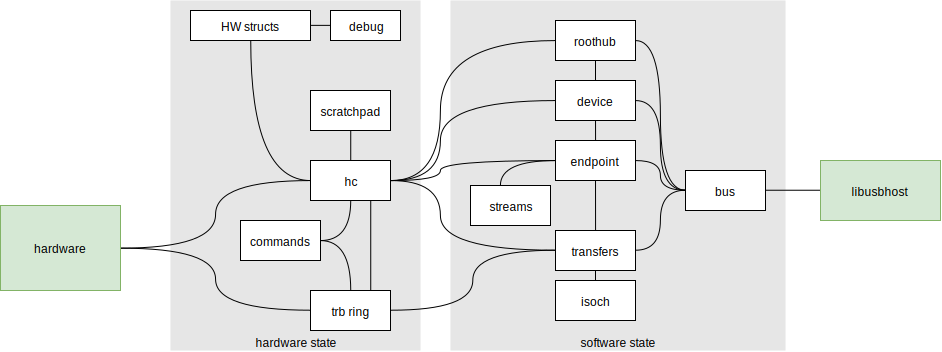
\includegraphics[width=0.8\textwidth]{xhci-architecture}
	\caption{The modules of xHCI driver}
\end{figure}

The scheme is not at all strict, we're in a C world, there are dependencies
almost everywhere -- take it as an informal overview to get an idea.

The whole driver can be split into two parts. The left one takes care of the
hardware perception of what's going on, the right one is about managing the
software structures and memory.

We start with describing the modules in the hardware part, as their
functionality is clear. Their order follows the order in which they were
implemented.

\section{Hardware Structures}

The \file{uspace/drv/bus/usb/xhci/hw\_struct}{hw\_struct} directory contains C structures
that represent registers and control structures used by the xHC. The memory layout of the
structures is defined by the xHCI specification\cite{xhci} and thus the files in this directory should
be mostly treated as read-only.

\subsection{Registers}

The register structures (defined in \file{uspace/drv/bus/usb/xhci/hw\_struct/regs.h}{regs.h})
represent hardware registers presented by the xHC to system software
implemented as Memory-Mapped I/O space. They can be divided into four categories as follows:
%
\begin{description}
	\item[Capability registers]
		These specify read-only limits, restrictions, and capabilities of the specific
		xHC implementation used.
	\item[Runtime and Operational registers]
		These specify the current xHC configuration and runtime modifiable state.
	\item[Extended capabilities]
		These specify optional features of the current xHC implementation.
	\item[Doorbell array]
		An array of up to 256 doorbell registers, which supports up to 255 USB devices
		or hubs. Each doorbell register provides the software with a mechanism for
		notifying the xHC if it has slot or endpoint-related work to perform.
\end{description}

In our implementation, all of these can be accessed through the \struct{xhci_hc_t} structure and
can be modified through it using the register handling macros defined in
\file{uspace/drv/bus/usb/xhci/hw\_struct/regs.h}{regs.h}. Note that not all register bits can be
manipulated freely by the system, some impose restrictions:
%
\begin{description}
	\item[RO, Read-only]
		Register bits are read-only and cannot be altered by system software. An example
		is the \textit{CAPLENGTH} register (see \xhci{5.3.1}).
	\item[RW, Read-Write]
		Register bits are read-write and can be altered by system software. An example
		is the \textit{USBCMD} register (see \xhci{5.4.1}), in which some bits or bit ranges
		are RW (and some are read-only).
	\item[RW1C, Write-1-to-clear]
		Register bits indicate status when read, a set bit can be cleared by writing
		a '1', writing a '0' to such register bit has no effect. An example is
		the \textit{Event Interrupt} bit in the \textit{USBSTS} register (see \xhci{5.4.2}) which is set
		to '1' by the xHC when an interrupt occurs and can be cleared by the driver
		by writing '1' to it once the event is scheduled for handling.
	\item[RW1S, Write-1-to-set]
		Register bits indicate status when read, a clear bit can be set by writing
		a '1', writing a '0' to such register bit has no effect. Examples are the
		\textit{Command Stop} and \textit{Command Abort} bits of the \textit{CRCR} register
		(see \xhci{5.4.5}).
\end{description}

This is not an exhaustive list of access attributes, for the entire list, see \xhci{5.1.1}.

\subsubsection{Register access macros}

Registers are accessed very often in all hardware-related modules. We felt that
there is a need to centralize the information defined in the specification,
especially the subdivision of registers to individual fields. There are several
common solutions to this problem.

Probably the most common one, which we also considered at first, is defining
two constants for every such field: mask and shift. When one needs to read
a field, they read the value of the register, use the mask to select bits, and
then shift the value according to the shift macro. To write a field, one reads
the value of the whole register, uses the bitwise negation of the mask to copy
surrounding bits, then shift the value to be written into its place. This
solution is simple to understand, yet hard to use correctly. There's a lot of
repetition, the more if you consider endianity (HelenOS is targeted also on Big
Endian platforms, while the USB world is Little Endian).

Another possibility is to define macros for reading and writing every single
field. That idea was discarded in its very beginning. We wanted a solution
that requires only one definition per field, cannot be used in a wrong way and
is sensibly short to write. So we came up with the register access macros. The
best introduction is probably by an artificial example:

\begin{listing}[h]
\begin{code}
#define XHCI_SOME_FIELD            usbreg, 32, RANGE, 13, 7

unsigned field = XHCI_REG_RD(hc->op_regs, XHCI_SOME_FIELD);
XHCI_REG_WR(hc->op_regs, XHCI_SOME_FIELD, 42);
\end{code}
	\caption[An example of using register macros]{On the first line, we read
	bits 13 to 7 of the field \mintinline{c}{hc->op_regs->usbreg} to
	a variable, and then change the same bits in the register to a value 42.}
\end{listing}

All the definitions of macros like \macro{XHCI_SOME_FIELD} relevant for xHCI
are contained in the header file \header|hw_struct/regs.h|. The definition
contains all the information necessary to access the field. It says that the
register field is contained in a field \struct{usbreg} of an operational
register structure (the one \mintinline{c}{hc->op_regs} points to), the
structure field is a 32-bit wide dword, and that the register field is
contained in bits 13 to 7 of it.

The primary principle used to implement these preprocessor macros is the
specific order of macro expansion in C. In the example, the register definition
macro is used as an argument to the \macro{XHCI_REG_RD} macro. Both macros are
expanded in a breadth-first fashion, producing just another preprocessor macro
\macro{XHCI_REG_RD_INNER(hc->op_regs, usbreg, 32, RANGE, 13, 7)}. You can see
that one argument is expanded to several arguments for the inner macro. What
happens next is pretty simple. The \macro{RANGE} argument token is glued to
a prefix, producing a name for another macro, which selects between
implementations for whole fields, bit ranges and individual bit flags. The
\macro{XHCI_REG_RD_RANGE} then extracts the specified bits read from the whole
field. The size argument is needed to properly handle endianity. All other
top-level macros (\macro{XHCI_REG_WR}, \macro{XHCI_REG_SET},
\macro{XHCI_REG_CLR}, \macro{XHCI_REG_MASK} and \macro{XHCI_REG_SHIFT}) operate
on the same principle.

We think we have achieved our goal. These macros are a bit hard to understand but
very easy to use and require just one line of definition per field. Looking
back though, the work was probably not worth it -- the registers are not used
that much to justify the existence of register definition of every single register
field. But it is already done and shall there be a need to access more registers,
it's easily accessible without thinking how to select the proper bits and
ensure the correct endianness. And even if there wasn't, it serves as a nice
showcase of what are preprocessor macros capable of.

\subsection{Contexts}

Contexts (defined in \file{uspace/drv/bus/usb/xhci/hw\_struct/context.h}{context.h})
are control structures that represent devices and their configuration as well
as the parameters of the communication between the xHC and system software. The
\struct{xhci_hc_t} structure contains the \textit{Device Context Base Address Array} (DCBAA), which
holds up to 255 pointers to device contexts at indices 1 through 255 and a pointer to
the scratchpad array (see \ref{sec:scratchpads}). Each device context contains a slot
context (used to describe the device as a whole, represented by \struct{xhci_slot_ctx_t}) and
31 contexts for each endpoint (represented by \struct{xhci_ep_ctx_t}). Most of these contexts
will be described in more detail in the following sections.

\section{Debug}

Since both the internal state of the xHC and its capabilities are often described by
a handful of bits located in a packed 32-bit register, we needed a way to monitor these
values in a human-readable form. The \file{uspace/drv/bus/usb/xhci/debug.h}{debug.h} and
\file{uspace/drv/bus/usb/xhci/debug.c}{debug.c} files contain a set of register dumping
functions that use the register reading macros described in the previous section to print
the values of all the bit sets contained in a register to the driver's log. They also contain
auxiliary functions that are used to convert numeric codes to their meaning in a string form and
functions that dump the contents of a hardware structure (such as \struct{xhci_endpoint_ctx}).

These functions have proved to be of great use and should any future maintainer of the
HelenOS xHC stack find themselves in a bug-ridden situation, putting these functions to
the areas of code they suspect of mischievous deeds might be a good starting point.

\section{TRB Ring}

One of the primary means of communication with the HC, apart from register
interface, are the TRB rings. Their management is fully contained in the TRB
ring module. Before we dive into the implementation details, let us first
describe how these rings works.

\subsection{Architectural overview}

\emph{Transaction Request Block}, everywhere else abbreviated as TRB, is
a fixed-size structure with contents of variable type. The most notable
exception being a \emph{TRB Type} field. Each of the 64 TRB types defines the
other fields that are contained inside a TRB. Most commonly, it just contains
a pointer to another buffer together with the size of the buffer, or a result
of an operation.

\emph{TRB Ring} is then a circular queue comprised of individual TRBs. The main
difference from older HCIs is that TRBs are required to be contiguous in
memory, forming a \emph{TRB Ring Segment}. It is of course needed to link the
two ends of the segment together, one must use a special TRB type called
\emph{Link TRB}, which serves as a glue between the end and the beginning of
a segment. It is not required from the ring to be composed of only one segment,
but then special precautions must be taken.

TRB Ring is used in many instances during the lifetime of the Host Controller.
There are two special instances though: the \emph{Command Ring} and the
\emph{Event Ring}. The command ring serves as a channel to command the HC, and
the command interface is described in more depth in section \ref{sec:commands}.
The event ring is asynchronously read to retrieve results of commands,
completed transactions and so on, as the primary information channel from HC to
host. Actually, there can be more than one instance of Event Ring, but that
requires the host to be able to recognise multiple interrupts, which is not
supported in the current version of HelenOS. The event subsystem is further
discussed in the section \ref{sec:events}. The third type of a~ring,
a~\emph{Transfer Ring}, is used for every pipe endpoint on the bus - either
Endpoint or a Stream. These are used by the Transfer module, described in
section \ref{sec:transfers}. For now, let's discover the mechanics of the rings
themselves, regardless of their type.

As already said, TRB ring is a circular queue. It always has one producer and
one consumer of TRBs. Every ring implicitly defines two pointers: the enqueue
pointer and the dequeue pointer. The producer uses the enqueue pointer to
enqueue TRBs and the consumer uses the dequeue pointer to dequeue them. The
pointers are not shared between the host and the Host Controller. Instead,
every TRB has one bit with special semantics, the \emph{Cycle Bit}. The
transition between values of TRB Cycle Bit of individual TRBs defines the
value of Enqueue pointer. An example situation is shown on the figure
\ref{fig:ring-simple}.

\begin{figure}[h]
	\centering
	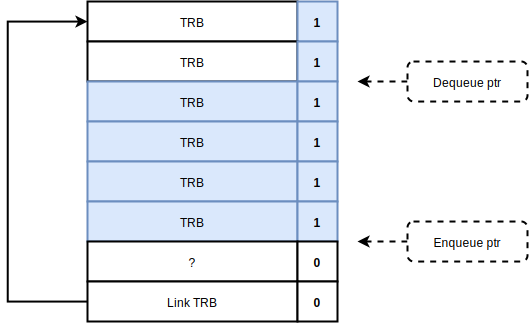
\includegraphics[width=0.6\textwidth]{ring-simple}
	\caption{A simple example of a TRB ring.}
	\label{fig:ring-simple}
\end{figure}

It is important to understand that the consumer cannot write to the ring and
thus cannot change the value of the Cycle Bit after it processes a TRB.
Therefore, the position of the dequeue pointer must be signalized by other
means. Furthermore, there has to be a mechanism to stop the consumer from
considering the TRBs in the beginning of the segment as enqueued, after it
wraps around the segment boundary. The enqueue pointer is not defined by
a transition from one to zero, but more generally by a transition from
\emph{Producer Cycle State}, \texttt{PCS}, to \texttt{\textasciitilde PCS}.
This bit is kept in the memory of the producer. Similarly, there exists
a \emph{Consumer Cycle State}, which has the same value as \texttt{PCS} had in
the moment when the value of the enqueue pointer was the same as the current
value of the dequeue pointer.

The Link TRB contains a \emph{Toggle Cycle} flag, which if set, instructs both
producer and consumer to toggle its cycle state when this TRB is
enqueued/dequeued (Link TRBs are not necessarily fixed in place, they are queue
members as any other TRB). There shall always be an odd number of Link TRBs
with the Toggle Cycle flag set on the ring.

We haven't yet covered how the producer can be aware of the dequeue pointer
value. In case of Command and Transfer rings, the producer is the Host
Controller. Every finished command or transfer is denoted by an Event TRB
placed on the Event Ring. This Event TRB usually contains the physical address
of the TRB on the respective Command or Transfer ring. This way the producer
knows that the dequeue pointer value is not less than the reported value.
Similarly, when the host processes an Event TRB on the Event Ring, it shall
report the physical address of the TRB processed by writing the value into
a dedicated register.

Also, the Event ring differs a bit in the usage of multiple segments. As the
Host Controller is obviously unable to allocate ring segments and map them into
virtual address space of the driver, and it's even not possible to allow the
host to write Link TRBs onto the ring, which is otherwise read-only for the
host, a~different approach has to be used. Instead of the segments being linked
together, the host preallocates a number of segments, and an \emph{Event Ring
Segment Table}, which is another structure defined by the specification. The
segments' addresses and sizes are written into the table, and the address of
the table is written to a dedicated register. At the time of the write, the
ownership of all the buffers is transferred to the Host Controller.

\subsection{Implementation}

As the requirements imposed by the specifications are quite strict, there's not
much freedom in the implementation. However, there were some decisions to be
discussed.

First, we decided not to restrict ourselves on single-segment rings as
other existing implementations do, though we haven't implemented runtime
scaling yet. Second, we implement and use three types of TRB rings;
the third one being a simplified TRB ring used by the host from both sides. Its
purpose is better described in the section \ref{sec:events}. The three
implementations are somehow separate, but because they share principles, they
reside in a common module.

The containing structures are called \struct{xhci_trb_ring_t},
\struct{xhci_event_ring_t} and \struct{xhci_sw_ring_t} for Command/Transfer
rings, Event ring and host-only rings, respectively. Despite their name, these
structures only represent the ring in host memory, and are not the structures
given to the hardware. Let's walk through them one by one.

\subsubsection{Command and Transfer Rings}

These rings are prepared to be multi-segment. They contain a list of
\struct{trb_segment_t} structures, which represent one ring segment. The
segment itself is allocated as a DMA buffer (sect. \ref{sec:dma-buffers}) of
size \macro{PAGE_SIZE}. The space for TRBs is in the beginning to ensure
alignment. At the end, there is a small footer keeping the physical address of
the segment and a link to the segment list. There are helper functions to
manage segments.

To avoid keeping the \struct{dma_buffer_t} structure inside the segment and
wasting precious DMA-accessible memory, the structure is reconstructed in order
to be freed in \fnc{trb_segment_free}. We agree that this violates the
encapsulation of DMA buffers, but consider this the lesser evil.

The main runtime interface to rings of this kind is the method
\fnc{xhci_trb_ring_enqueue_multiple}, used to enqueue a contiguous array of
TRBs (referred to as Transfer Descriptor, TD) onto the ring. As this method
must not block to be usable in atomic contexts, it first performs a dry run to
check if there is enough space on the ring, then rollbacks and actually
emplaces the TRBs. Because it might be needed to interleave the Transfer
Descriptor with multiple Link TRBs, it is not possible to simply calculate the
free space in advance.

Because the caller of this function needs to know the physical address of the
TRB enqueued to pair it with the completion event, the address is assigned to
an output argument. If there are multiple TRBs to be enqueued, the one with
\emph{Interrupt On Completion} flag is reported -- because that's the one that
will generate the event.

The second crucial part of the interface is the function
\fnc{xhci_trb_ring_update_dequeue}, by which the dequeue pointer advancement is
announced to the ring. As the rings need to be configured to the hardware
somehow, there is also a function called
\fnc{xhci_trb_ring_reset_dequeue_state}, which is used to reset the ring and
also return a value used to configure the ring in the HC -- a physical pointer
mixed with the initial Consumer Cycle State.

\subsubsection{Event Ring}

The implementation of the event ring is fairly simple, with the main
interaction point being the function \fnc{xhci_event_ring_dequeue}. This
method, symmetrically to the TRB ring enqueue, does not block if the ring is
empty, but returns \macro{ENOENT} instead. This structure also contains the
Event Ring Segment Table.

\subsubsection{Software Ring}

This structure is to be used as a buffer for exchanging information between
different fibrils of the driver. It is an ordinary implementation of a circular
blocking queue made for TRBs. It uses the Cycle bit inside TRBs to indicate
active entries, because both sides are allowed write to the ring when the guard
is locked. Also, this ring is not allocated using DMA buffers, because it is
not expected to be accessed by hardware.


\section{Scratchpad}
\label{sec:scratchpads}

Scratchpads are buffers that an xHC implementation can request from the system software
for its internal needs. The size of these buffers is specified in the \textit{PAGESIZE} register
found in the operational register set defined in \struct{xhci_op_regs}.

The amount of buffers requested by the xHC is specified in the \textit{Max Scratchpad Bufs Hi} and
\textit{Max Scratchpad Bufs Lo} registers of the second set of structural parameters (\textit{HCSPARAMS2},
see \xhci{5.3.4}) defined in \struct{xhci_cap_regs}.

The allocation of these buffers takes place as part of the host controller initialization,
specifically in \fnc{hc_init_memory}, which calls \fnc{xhci_scratchpad_alloc}. The pointers
to these buffers are then passed to the xHC in the \textit{Scratchpad Buffer Array}, pointer to which
occupies the first index of the \textit{Device Context Base Address Array} (dcbaa field of
\struct{xhci_hc_t}).

Our implementation originally implemented these as a standalone structure \struct{xhci_scratchpad_t},
which served mainly for the purposes of resource management by keeping both the physical addresses
for the xHC and the virtual addresses for deallocation. This was, however, later refactored to use
\struct{dma_buffer_t}, which is part of \lib{libusbhost} and was created for the same purpose.

Once the xHCI driver finishes its execution, the scratchpad buffers are deallocated by a call to
\fnc{xhci_scratchpad_free} as part of \fnc{hc_fini}.


\section{Commands}
\label{sec:commands}

The xHC offers an independent command interface. During operation, the xHC
driver uses this interface to manipulate device slots, devices and endpoints by
executing various commands provided by a unified command subsystem. This
section provides details on the structure and implementation of this subsystem.


\subsection{Execution Workflow}

The xHC command interface consists of a TRB command ring and a command doorbell
register. Commands are executed by placing various command TRBs onto this ring,
forming a \textit{Command Descriptor}.

After placing the respective TRBs and writing to the xHC command doorbell
register, the descriptors on the command ring are sequentially processed by the
xHC, resulting in either failure or successful completion. The result of every
command descriptor is reported back to the xHCI driver in the form of a
\textit{Command Completion Event} placed onto the primary event TRB ring.

After writing into the xHC command doorbell register and before receiving the
respective command completion event, the xHCI driver can attempt to abort the
issued command. Such action might be of use for instance if the command
completion event does not arrive within a set time period.

Note that this section intentionally omits hardware technical details, which are
not instrumental in understanding the command subsystem. For further hardware
documentation of the xHC command interface, refer to \xhci{4.6}.


\subsection{Structure}

The xHCI driver command subsystem instance is represented by the
\struct{xhci_cmd_ring_t} structure which exists throughout the entire duration
of the xHCI driver's lifecycle. The purpose of this structure is to maintain and
manage the command TRB ring and to keep track of enqueued command descriptors.

Individual command descriptors are represented by the \struct{xhci_cmd_t}
structure. In this structure are stored high-level parameters of the command as well as
the command TRB, which is placed onto the command ring when the command is
executed. While the high-level command parameters are kept directly in this
structure, the hardware-related internals are kept in a substructure, which is
commonly referred to as \textit{command header}. The purpose of this separation
is to stress that the header contents are to be exclusively accessible to the
command subsystem, while the rest of the structure remains accessible to
the entire xHCI driver.

Besides data structures, the command subsystem offers a centralized command
completion event handler function -- \fnc{xhci_handle_command_completion} --
which is called by the event subsystem in case a \textit{Command Completion
Event} is encountered.

The last major component of the command subsystem are functions used to generate
and schedule commands on the xHC. These functions produce valid instances of the
\struct{xhci_cmd_t} and place their respective TRBs onto the command ring
managed by the \struct{xhci_cmd_ring_t} structure, requesting either blocking or
non-blocking semantics for waiting on their completion. These functions are
described in detail in the next section.


\subsection{Command Lifecycle}

\subsubsection{Issuing Commands}

By design, the internal logic of the command subsystem is kept opaque with
respect to other components of the driver. A notable example of this is the
mechanism for command scheduling.

Commands are usually issued by the HC component of the xHCI driver. At the time
of issuing, the information required can be broken down into three groups:
%
\begin{description}
	\item[Command Type]
		One of the 15 commands supported by the xHC command interface.
	\item[Command-specific Parameters]
		The number, type and semantics of these parameters depend on the
		specified command type.
	\item[Completion Semantics]
		This is the desired behavior of command execution.

		In the \textit{blocking mode}, the call to issue the command will block
		the calling fibril until the completion event is received.

		On the other hand, in the \textit{non-blocking mode}, the fibril will
		only be blocked until the command is issued -- the command subsystem
		will take the ownership of the command and deallocate it when the
		completion event arrives. This mode is meant for commands which do not
		require completion event handling and involves more complicated memory
		management since the command subsystem is responsible for freeing the
		command after the completion occurs.
\end{description}

Depending on the desired completion semantics of the issued command, the HC
component calls either the \fnc{xhci_cmd_sync} or \fnc{xhci_cmd_async}
function and passes it a configured instance of the \struct{xhci_cmd_t} structure.
Upon such call, the command subsystem will execute an internal command handler
function, which copies the high-level command-specific parameters configured by
the issuer, and use their values to construct a command descriptor consisting of
TRBs.

At this point, the \struct{xhci_cmd_ring_t} structure is modified and the new
command descriptor is placed onto the TRB ring. The corresponding instance of
\struct{xhci_cmd_t} is added to the active command list and depending on the
completion semantics, the issuing fibril is either suspended or continues
execution regardless of the completion event.


\subsubsection{Handling Completion}

When a command is completed, a \textit{Command Completion Event} is generated by
the xHC. This event is detected by the event subsystem, which in such case
triggers the \fnc{xhci_handle_command_completion} function.

This function extracts the address of the completed command descriptor and uses
it to find a matching instance of the \struct{xhci_cmd_t} structure in the
active command list.

Depending on the desired completion semantics, the command subsystem either
wakes the sleeping issuer fibril, or discards the non-blocking command from the
memory.


\subsubsection{Aborting Commands}

The command subsystem defined by xHCI contains a mechanism to trigger early
command abortion. It is not guaranteed to be effective for all commands, just
for commands control of which is out of HC's hands. A good example might be the
\macro{SET_ADDRESS} command, which issues the USB control request
\emph{SetAddress}, and waits for the device's response. Such command blocks
until the response is received. If the software, for any reason, wants the
command to be aborted, it can write 1 to the \macro{CA} bit of the
\emph{Command Ring Control Register}.

When the HC is triggered by a command abortion, it places a \emph{Command Ring
Stopped} event on the primary event ring and halts command processing. The ring
can be started again by ringing its doorbell. If a command was actually
aborted, a corresponding \emph{Command Completion Event} with status
\emph{Command Aborted} is placed first.

We decided to set a fixed timeout for every command, regardless of its
possibility to block, arbitrarily chosen as 10 seconds. That gives a generous
amount of time for the HC to finish a command. When this timeout is over,
a command is aborted.

Here comes the catch: the driver is not able to choose which command is to be
aborted -- it is always the one currently processed. Usually, it's the one that
blocks the pipe, but it means that the driver cannot simply place a timed
constraint on a command execution. To reflect the hardware semantics, all
fibrils that expire the timeout behave the same: they trigger a command
abortion, wait for the command ring to be stopped, then start it again.

To orchestrate several fibrils trying to schedule new commands, waiting for
commands to be completed and also the one handling an interrupt, a simple state
machine with synchronization is incorporated. In case the command ring is
being restarted, newly issued commands are delayed to prevent the doorbell from
being rung unexpectedly. When there are multiple fibrils with an expired timeout
while the abort is already triggered but not yet finished, they retract and
wait for the full timeout period again.

That common execution path is enclosed within a function called
\fnc{try_abort_current_command} (static for the command subsystem). As it's hard
to force a command to stall, we haven't had many opportunities to test the
behavior. Usually, the mechanism was triggered by a deadlock in our code, which
didn't magically disappear when a command was aborted. Also, the commands
always finish on time in a virtual environment. At the time of writing this
documentation, there has been only one observed legitimate occurrence of
a command stall on real hardware. The abort mechanism did its job well that day.

\subsection{Usage Examples}

Since the command subsystem is used at a multitude of places in the HC
component, it has been the goal of the authors to make its usage elegant and
effortless. For that reason, a dedicated inline notation syntax powered by
preprocessor macros has been devised and implemented. This is demonstrated in
Listing \ref{lst:command-usage}.

\begin{listing}[h]
	\begin{code}
		xhci_hc_t * const hc;

		/* Issue a "Set TR Dequeue Pointer" command synchronously. */
		const int result = xhci_cmd_sync_inline(hc, SET_TR_DEQUEUE_POINTER,
		    /* Command-specific arguments use struct initializer. */
		    .slot_id = slot_id,
		    .endpoint_id = dci,
		    .stream_id = stream_id,
		    .dequeue_ptr = addr,
		);

		/* At this point, the command is completed with `result`. */
	\end{code}
	\caption[Usage example of xHCI driver inline command syntax.]{Usage example
	of the xHCI driver command subsystem inline  syntax. This snippet issues a
	\textit{Set TR Dequeue Pointer} command to the HC in blocking mode. Note
	that the command initialization, configuration and finalization is handled
	by the inline macro syntax.}
	\label{lst:command-usage}
\end{listing}



\section{Host Controller Module}

This module contains the mixture of things that didn't fit anywhere else or
didn't deserve their own submodule. We tried to move the ``xHCI specification
quirks'' here, so that other modules rely only on the semantics and overview of
the xHCI, and don't care that much about the exact technical details. Of
course, it's not strictly possible, because the whole driver is about technical
details of xHCI.

\subsection{Initialization}

A substantial part of this module handles the initialization of the controller.
When the xHC device is added, several steps need to be done. Let's walk through
them in order. The DDF callback \fnc{dev_add} is handled by the
\lib{libusbhost} library, so the story begins there.

\begin{enumerate}
\item
	At the very beginning, the supplementary structures are allocated in the
	DDF device node. These structures accompany the entire lifetime of a driven
	HC.

\item
	The DDF control function is created. Through it, the user may command the
	HC driver.

\item
	The hardware resources such as MMIO space or IRQ number are obtained from
	the parent device (usually PCI driver).

	Now, the structure and hardware resources are handed out to the xHCI driver for
	the first time, to do its initialization.

\item
	The MMIO range needs to be mapped, and the proper register areas found.
	xHCI specifies several areas of MMIO registers, with variable offsets
	between them. We cache the pointers to the areas inside the
	\struct{xhci_hc_t} structure to make the access convenient.

\item
	The roothub structures are initialized. The number of ports is obtained and
	memory for state machines is allocated.

\item
	Extended capabilities need to be parsed soon enough, as they contain some
	crucial information. Namely the information about legacy support, but also
	the protocol versions supported on individual roothub ports.

\item
	A lot of memory structures are to be initialized now. The \emph{DCBA}
	array, event ring, scratchpads, command ring, the device-keeping array and
	also the event worker fibril.

	After all of that, the basic driver initialization is completed, and the
	execution returns to the library.

\item
	The interrupts need to be enabled if they are available. The driver is
	given an opportunity to generate the bottom-half IRQ handling code, and
	then the code is registered in the kernel. Shall any of these steps fail,
	the failure is not critical and the interrupts are just marked unavailable.

\item
	If the HC is being controlled by the BIOS (denoted by the extended
	capability), it needs to be claimed.

\item
	The HC is started. In case of xHCI, an initialization sequence as described
	in the specification is performed. The HC is reset to transition into
	a known state. The addresses of the memory structures are configured. If
	the interrupts are available, the interrupter 0 is enabled. Finally, the HC
	is started by setting a bit in the operational registers.

\item
	Before the control is returned to the library, all roothub ports are
	checked for a change, because the reset changed their connection state,
	but the Port Change Events had no ring to be written on.

\item
	If the interrupts are not available, a replacement polling fibril is
	started.

\item
	The roothub is to be set up. Other HCs using virthub must undergo an
	enumeration process, so this must be done after the initialization is fully
	completed. In the case of xHCI, this step is skipped.
\end{enumerate}

A symmetric reverse sequence is performed to make the HC stopped again. This
functionality is however not tested because PCI devices are not hotpluggable,
not even in QEMU.

\subsection{Events}
\label{sec:events}

Another functionality provided by the HC module is the first line of handling
events. Events are the primary information channel from the device to the host.
Every synchronous operation needs to be finished by waiting for an event.

The tricky part in handling events is, again, the synchronization. Event
handlers must not issue operations, which would wait for other events. The
problem is that this event dependency is inevitable in some cases. Let us
describe two scenarios which will explain the complexity of the final solution.

First, there are the Port State Changed Events. Handling these events usually
involves device enumeration -- that is however handled in a separate fibril.
It's even not the reset completion which would create a deadlock -- if it is
expected, all the locks are unlocked. The main problem is a device
disconnection while the enumeration is still in progress -- when it happens,
the event handling fibril must wait until the enumeration fibril terminates.
But the enumeration might be in the later phase, in which it issues commands.
In order to terminate, a command must be completed. That introduces
a dependency, which cannot be simply removed. Because of it, Port Change
Detected Events and Command Completion Events must be handled independently on
each other.

Similarly, the enumeration process involves fetching descriptors from the
device. That introduces another dependency, this time between Transfer
Events and Port Change Detected Events. Neither these two can be handled
sequentially.

The last dependency is between Command Completion Events and Transfer Events,
forming a dependency triangle. This one might not be that obvious, but it is
there and cannot be avoided easily. The handler of the Transfer Event needs to
obtain a reference to an endpoint. To ensure coherency, the reference must be
created while the endpoint is still registered, in a critical section. The same
critical section that protects the endpoint unregistration -- which needs to
abort currently running transfers.

In order to avoid a deadlock, all three types of events need to be processed
separately. We achieve that by processing only so-called fast events (Command
Completion, MFINDEX Wrap) in the interrupt handler, and route the Port Change
Events and Transfer Events to two Software TRB Rings (see section \ref{sec:sw-rings}),
from which two other worker fibrils dequeue and handle the events independently.

\subsection{Commands abstraction}

Although the command interface has a module on its own, there are situations
where the specific commands used are a technical detail hiding the actual
semantics of the operation. To give an example, to inform the HC about dropping
an endpoint, one must issue the \emph{Configure Endpoint} command with a flag
set. Also, some commands require an input context with a proper content, some don't.

The rest of the Host controller module tries to cover these implementation
details and offer a more intuitive interface. Although the device and endpoint
modules do fill the contexts on their own (being also a technical detail), the
decision whether it's needed to fill an input context is left to the HC module.

\section{Root Hub}

The purpose of this module is very simple -- take care of the root hub. Before
we explain how our roothub works, let's have a look at why and how other HC
drivers handle it.

The main problem a hub driver faces is a synchronization one. When a new device
is detected, it needs to be enumerated. Enumeration process in the case of USB 2.0
devices requires the hub to reset the port the device is attached to in order to move
it to the \state{Default} state when it's listening on the default address 0.
When the port reset is triggered, the hub must wait until the port reset is
complete. During the whole process the device can be disconnected and the
port reset will never be completed. Furthermore, the completion of the port reset
is indicated by the same means as port connection, resulting in a deadlock in
the na\"ive solution. The proper solution therefore involves spawning new
fibrils and nontrivial synchronization.

All four HC drivers (UHCI, OHCI, EHCI, and VHC) are using a virtual roothub. In
principle that means that they create a virtual USB device, which is listening
on the default address in the beginning, and trigger an enumeration process.
Then there is a little branch in transfer scheduling, that takes transfers
directed to the same address as the virtual device's, and delivers them by
calling a function instead. The virtual device behaves exactly like a real USB
hub would -- it has its standard descriptors, replies to setup requests and so
on. So it enumerates like a USB hub would and creates a DDF device, which is
taken by the \texttt{usbhub} driver. The driver then handles the virtual
roothub like any other hub -- by sending USB control transfers. The virthub
module translates USB transfers to callbacks, which are implemented by the
individual HC drivers to read and modify register space of the Host Controller.

This solution is very clean in design, regarding that root hub functionality is
exactly the same as any other hub's, but just controlled by MMIO mapped
registers instead of USB packets. It is even recommended by the USB 2.0
specification \cite{usb2} to embody this solution. But that's pretty much the only advantage
this solution has. One has to write a lot of code to even implement the
callbacks, not mentioning the virthub module itself. And a lot of code always
comes with bugs. Also, while having no real performance impact, it requires
several context switches, IPC calls, bouncing memory buffers and a lot of
unnecessary allocations to clear one bit in the register space (USB hubs
operate by setting and clearing so-called Features, indicating e.g.\ that
a connection on port changed). But it needs to be stressed more that this
performance impact is mitigated by the fact that real hubs use real USB transactions
above that and that hub interaction is very sparse.

We searched for a solution that would keep the cleanness in terms of shared
functionality between usbhub driver and roothub and decided to move the port
state machine and related fibril synchronization into the USB library. That
cleanly separates the hardest part of handling hub port changes from the code
that is actually handling them and enumerating the devices. This state machine
is used by both the xHCI roothub and also by the rewritten usbhub. More
information about this new module can be found in section \ref{hub-port-refactoring}.

One more thing related to the xHCI roothub, which we crossed while debugging on
real hardware: the USB hub has a bit dedicated to indicate that a port is
enabled (PED), and the port can be disabled using it. Counterintuitively, the
port is disabled by writing a 1 to it. Even worse, this bit is in the same
field as the change bits with RW1C semantics are -- which means that the
standard approach of reading and writing back the value read fails hard. This
took us several hours to discover because the port reset was completed
successfully, but right after that, the device was inaccessible, even when we
didn't do anything with it yet. To make matters more complicated, QEMU ignores
this bit completely so the code worked fine in a virtual environment.

\section{Bus Module}

% TODO: After the device will be split, will there be anything interesting to write about?

\subsection{Device}

Devices in the xHCI are represented by structures called device contexts, these are
managed by the xHC and used to report device configuration and current state. A device
context consists of a slot context, which represents the device as a whole (e.g. contains
information about addressing or power management) and is implemented in the \struct{xhci_slot_ctx_t}
structure, and 31 endpoint contexts (which are described in the following section)
for each of the device's possible endpoints (though most of them may never be used).

Note that one will not find a specific structure used to represent a device context. We had
one at first, but later discovered that according to a note in section 6.2.1 of the
specification, the \textit{Context Size} field in the \textit{HCCPARAMS1} register determines whether
a device context contains 32 or 64-byte members (the size of the individual members does
not change, but the 64-byte version adds 32 bytes wide padding to each of them). Because
of this, the device context structure cannot be represented statically and instead had to be
implemented as a DMA buffer (see section \ref{sec:dma_bufs}) and its members have to
be accessed dynamically at runtime.

A device is initialized during a process called device enumeration, which begins when
the system detects a new device and calls \fnc{xhci_device_enumerate} defined in
\file{uspace/drv/bus/usb/xhci/device.c}{device.c}. This function then initializes the device
by requesting its slot (index to the \textit{Device Context Base Address Array} field in
\struct{xhci_hc_t}), enabling and configuring its control endpoint and requesting
an address for it.

\subsection{Endpoint}

% TODO: Contexts, rings

\section{Transfers}
\label{sec:transfers}

The xHC uses transfers to abstract USB communication. Every call to
\fnc{usb_write} and \fnc{usb_read} is accomplished by creating a transfer,
setting it up, handing it to the xHC and waiting for transfer completion. This
section describes the code structure and implementation details of the xHCI transfer
subsystem.

\subsection{Executing Transfers}

The xHC is responsible for communicating with USB devices using USB packets.
These USB packets are created from the data given to the xHC through the
transfer rings by the software. The software isn't required to split the
transfer into USB packets, the xHC takes care of that.

Each transfer is formed by a \textit{Transfer Descriptor}, which is a sequence
of TRBs with a chain bit set. This allows the software to schedule a transfer
containing larger data, or data not stored in continuous memory. Each TRB
points to a single continuous buffer of data (in physical memory) and specifies
the buffer's size. This buffer must be accessible to the hardware and it's
physical address needs to be set to the TRB.

Every endpoint uses a single transfer ring (with the exception of streams)
initialized during the endpoint configuration. This transfer ring is passed to
the xHC by the endpoint context. The software is not allowed to modify the
transfer ring except when it wants to enqueue more transfer descriptors. If the
software requires to modify the ring, it has to first stop the endpoint using
the command interface, and after the modification is done, it has to use the
evaluate context command to communicate the changes to the xHC.

After the software puts a transfer descriptor on the transfer ring, it rings
the doorbell associated with the device and the endpoint. This notifies the xHC
and causes it to schedule the endpoint and process the transfer.

After the transfer descriptor finishes processing, the xHC can optionally
notify the software of the completion by generating a \textit{Transfer Event}
on the event ring with the completion code set to reflect the result. By
default, this only happens if the TRB processing ends with an error.
The software can set the \textit{IOC (Interrupt on Completion)} bit if it needs
to be notified regardless of an error happening.

\subsection{Lifecycle}

Every transfer is represented by a single instance of \struct{xhci_transfer_t}
structure. This structure encapsulates the \struct{usb_transfer_batch_t}
structure, which is used by \lib{libusbhost} to schedule USB batches. Its
lifetime is managed by the library calling the bus operations.

After the library allocates and fills up the \struct{usb_transfer_batch_t}, it
schedules the transfer. This is where the xHCI takes control over the transfer.
The transfer is processed in \fnc{xhci_transfer_schedule}, where it is split
into TRBs, the correct bits are set depending on the transfer type, TRBs are
enqueued and the doorbell is rung.

The fibril responsible for this transfer then waits for the transfer event
signalizing that the transfer has finished. This means that the IOC bit is set
for every transfer descriptor so that the software gets notified about its
completion.

After the transfer event is received, the event loop calls
\fnc{xhci_handle_transfer_event}. There, the TRB which triggered the event is
processed and the transfer, that scheduled it, is found. For IN endpoints, the
received data is copied to prepared buffers. In the end, error code is set in
the batch and the batch is finalized.

\subsection{Isochronous Transfers}

Due to the nature of isochronous transfers, their implementation needs to avoid
the common steps used by other transfers. This section describes the
requirements and details of the isochronous transfer support.

The xHC has an internal timer and it measures time in \textit{microframes},
where 1 microframe is exactly 125 microseconds. The current time in microframes
can be read anytime from the \texttt{MFINDEX} register. This register has only
14 bits and therefore it wraps every 2.048 seconds. The xHC can notify the
software about the wrap by generating a \textit{MFINDEX Wrap Event} on the
event ring. This feature is optional and must be enabled beforehand.

Every isochronous transfer descriptor must have a set schedule time. This time
is calculated by the software and depends on the isochronous endpoint interval.
Two following transfer descriptors must be always exactly the interval apart.
Because the isochronous endpoints can have up to 4 second interval, we need to
track the \textit{MFINDEX Wrap Events} to correctly determine the scheduling
time.

The xHC gives software strict deadlines when an isochronous transfer descriptor
may be present on the transfer ring for the transfer to execute successfully.
This interval is partially HC specific and it's based on \textit{Isochronous
scheduling interval} (IST). The transfer must be present on the ring at least
\textit{IST} microframes and at most 895 milliseconds before it is to be
executed.

The isochronous endpoint also reserves some bandwidth during its setup and has
only its reserved bandwidth available, therefore the xHC never permits using
more bandwidth. This sets a hard cap on the size of the data transferred in a
single transfer descriptor. Scheduling a transfer descriptor with larger data
causes the xHC to generate an error and refuse to transfer the data.

If the xHC accesses an isochronous transfer ring to retrieve a transfer
descriptor and the transfer ring is empty, the xHC generates a Transfer Event
with the completion code set to \textit{Ring Overrun} for IN endpoints, and
\textit{Ring Underrun} for OUT endpoints. This also removes the endpoint from
the schedule and lets software clean the structure and report the error to the
driver, if needed. To reschedule the endpoint, the software needs to ring a
doorbell.

\subsubsection{Implementation}

When we were implementing isochronous transfers, we had to consider all the
requirements described above. We tried to not introduce an API specific for
isochronous transfers to not clutter the interface.

To maintain the \lib{libusbhost} API, we have decided to slightly change the
semantics of calling \fnc{usb_write} and \fnc{usb_read} on isochronous
endpoints. The \struct{xhci_endpoint_t} structure includes a substructure for
fields specific to isochronous endpoints in \struct{xhci_isoch_t}. There is a
small trick present to avoid inflating the \struct{xhci_endpoint_t} for every
type of endpoint. The last field of the structure is a zero length array of
\struct{xhci_isoch_t}. This doesn't take any space, but the pointer to this
field is always valid and points behind the structure. We then allocate the
structure with \texttt{calloc(1, sizeof(xhci\_endpoint\_t) + (type ==
USB\_TRANSFER\_ISOCHRONOUS) * sizeof(*ep->isoch))}. If the endpoint is
isochronous, the memory allocated is larger to accommodate the
\struct{xhci_isoch_t} and we use the pointer mentioned previously to access it.

The \struct{xhci_isoch_t} also contains a dynamic array of
\struct{xhci_isoch_transfer_t}. These represent an isochronous transfer and
maintain a permanently allocated data buffer. The amount of these depends on
the IST and the endpoint interval as we need to make sure we put the transfer
descriptors on the transfer ring in advance, but do not schedule too old data.

\subsubsection{IN endpoints}

For IN endpoints, the semantics of \fnc{usb_read} are changed so that instead
of triggering a read transfer, the call retrieves previously read data and
returns them to the caller. This means that we have to enqueue read transfers
in advance and the caller is expected to withdraw them fast enough. If there is
no prepared data, the call blocks waiting for them instead of returning an
error.

To keep the transfer ring filled with transfer descriptors, we prepare a
transfer descriptor for every transfer buffer when the first read is called and
enqueue as many as possible to the transfer ring before ringing the doorbell
for the first time. This means that not all descriptors may be enqueued because
of the strict deadlines described above. If this happens, we start a timer,
which takes care of putting the transfer descriptors on the ring when the time
is right. After every call to \fnc{usb_read} and withdrawing the received data,
the processed buffer is recycled and scheduled back on the transfer ring.

\subsubsection{OUT endpoints}

For OUT endpoints, the \fnc{usb_write} doesn't ensure that the transfer
finishes. Instead, it only copies the data to the buffer and attempts to put
the buffer on the ring, if possible. If there is no free buffer yet (so all the
buffers are on the ring), the call blocks until at least one transfer is
finished and its buffer is freed.

Unlike with IN endpoints, we need to track, which buffers are filled and which
are empty, and schedule only filled buffers. Other than that, the scheduling is
the same. When scheduling the buffers at the start, we also need to make sure
some of those are already ready on the ring, so we postpone the execution of
the first transfer descriptor by a short delay.

\subsubsection{Error handling}

The transfer errors in isochronous transfers are very often not considered fatal
and should be skipped. Therefore, we decided to not deliver the
error to the driver immediately, instead, the error that occurred is returned with
the next \fnc{usb_read} or \fnc{usb_write} call, in the \texttt{error} field of
\struct{usb_transfer_batch_t}.

On the other hand, the \textit{Ring Overrun} and \textit{Ring Underrun} errors
are considered fatal as there is no simple way to recover from them. For IN
endpoints and therefore for \textit{Ring Overrun}, the error tells us that the
driver either cannot keep up and read the data fast enough, or it has stopped
reading completely. To not preserve old data, we reset the state of our
internal buffers. If the driver attempts to read again, the transfers are
started again as if the endpoint was accessed for the first time.

For OUT endpoints and \textit{Ring Underrun}, this means that the driver cannot
supply data fast enough or it has stopped sending them. We reset the endpoint
again and restart if the driver writes to the endpoint again.

Unfortunately, some host controllers (or QEMU, at least) don't generate
\textit{Ring Overrun} and \textit{Ring Underrun} events. We have therefore
implemented a mechanism to detect the issues these events convey ourselves.
There is a \textit{reset timer} for each isochronous endpoint that is started
every time a buffer is added to the ring, or a transfer event is received. The
timer is set to expire after the endpoint interval passes plus a small
constant. If this timer expires, we know that there was no event for at least
the endpoint interval and therefore the endpoint isn't working properly, so we
consider this as the error and reset the endpoint.

\subsection{Streams}

% TODO @salmelu: Noone else understands that now.


\chapter{USB Subsystem Modifications}
\label{usb-refactoring}

% TODO

\section{Explicit Device Removal}

One of the project goals is to alter the USB subsystem to allow support for
explicit device removal. Such feature can be found in most modern operating
systems and is often used to ensure that devices are left in a consistent state
after a physical port detachment occurs.

The explicit device removal feature usually provides a frontend interface in
the operating system, through which users can observe currently connected
devices and, if needed, issue a signal to the operating system that their
physical detachment is imminent. Following that, the system is expected to
promptly terminate all ongoing communications with the device and signal the
user back. After receiving the confirmation, user can then safely unplug the
device from the system bus without any risk of interrupting communications,
which could otherwise result in undefined state of the device.


\subsection{Considerations}

In the USB protocol, communications between the host and the device take place
in the form of \textit{transfers}. Depending on its version, the host controller
may have various roles in the realization of these transfers. For that reason,
version-specific modifications are carried out separately in host controller
drivers, whereas common functionality is implemented in the bus module, which is
a part of \lib{libusbhost}.

The disconnection routine for explicit device removal is implemented as follows:
~
\begin{enumerate}
	\item The user signals the intention to disconnect a USB device.
	\item The respective device drivers are notified to end their business (e.
		g. flush buffers or close files), possibly scheduling a multitude of
		transfers to the device.
	\item The HC driver disables the capability to schedule new transfers to the
		device.
	\item The HC driver aborts all leftover active transfers to the device.
	\item The device configuration is dropped, leaving it in the
		\state{Addressed} state, in which it is considered safe to be
		physically removed from the bus.
\end{enumerate}

If the user requests that this routine is rolled back, the steps of the
disconnection routine are just executed in reverse order. The following can
therefore be labeled as a reconnection routine:
~
\begin{enumerate}
	\item The user signals the intention to resume communications with a USB
	device, on which the disconnection routine has been previously performed.
	\item The HC driver configures the device.
	\item The HC driver enables the capability to schedule new transfers to the
	device.
	\item The operating system is notified that the device is reachable and
	matches it to appropriate drivers, which initiate communications with it.
\end{enumerate}

The specialization of both routines is performed in the same way as other bus
module interactions. All HC drivers hand off their DDF and device callbacks to
the bus module, which then calls them back to perform low-level commands related
to specific devices, endpoints and transfers. This way, the high-level logic
contained by the bus module essentially follows the listed descriptions above
and the version-specific extensions are resolved in the respective HC driver
implementations.


\subsection{Offline and Online DDF Signal}

The HelenOS Device Driver Framework includes two user-initiated signals
relevant to the implementation of this feature.

\begin{description}
	\item[Offline Signal]
		This signal informs a driver attached to a DDF node that its managed
		device may be removed in the near future. The driver is expected to
		immediately cease all user operations on the device and unbind its
		child DDF functions, possibly sending a \textit{Device Remove} signal
		to all their attached drivers in the process.

	\item[Online Signal]
		This signal is a logical counterpart to the previous signal.
		It informs a driver attached to a DDF node that its managed device will
		not be removed in the near future. The driver is expected to expose all
		child DDF functions related to the device, possibly sending a
		\textit{Device Add} signal to all their matched drivers in the process.
\end{description}

These signals can be easily issued by the user from the system shell by means
of the \app{devctl} application. See Listing \ref{lst:devctl-offline-online}
for invocation example.

\begin{listing}
	\begin{bdsh}
		# Prepare the unplug high speed device at address 2.
		devctl offline /hw/pci0/00:04.0/usb2-hs

		# We changed our mind. Bring the device back online.
		devctl online /hw/pci0/00:04.0/usb2-hs
	\end{bdsh}
	\caption[Example usage of \app{devctl} to issue offline and online
	signal.]{Example usage of the \app{devctl} application to issue offline and
	online signal to a USB high speed device at address 2. The host controller
	PCI address is \texttt{00:04.0}.}
	\label{lst:devctl-offline-online}
\end{listing}

It follows that these signals can be used for the implementation of the
explicit device removal at the level of USB host controller drivers. For that
reason, \lib{libusbhost} has been extended to handle appropriate DDF callbacks
for functions corresponding to HC's child devices. Their handling is forwarded
to the bus module, which executes the disconnection or the reconnection routine
for the \textit{offline} and \textit{online} signal respectively. In addition,
the transfer scheduling mechanism of the bus module has been extended to permit
scheduling new transfers only to devices, which are in the online state.

The general scheme of stopping communication with a device breaks down to
unregistering all its registered endpoints. The biggest challenge the driver
faces is to abort all currently running transfers on an endpoint that is being
unregistered. The majority of transfers (Bulk, Control, Isochronous,
Interrupt-out) wouldn't pose a problem -- we could just wait the short while
until they are completed, either successfully or not. But then there are
Interrupt-in transfers, which, especially in case of gone device, may not
complete in a timely manner.

\subsection{Aborting active transfers}

It is not possible to ``abort a transfer'' in a generic way, mainly because of
synchronization issues. Before we explain how can a transfer be properly
aborted in various Host Controllers, let us describe the lifecycle of
a transfer batch, a structure representing a transfer in HC drivers.

Currently, USB stack in HelenOS only supports synchronous interface to interact
with pipes. The two methods are called \fnc{dev_read} and \fnc{dev_write}.
Driver calls these methods on pipes, and provides a buffer -- either filled
with data, or to be filled. Once the call crosses the IPC barrier, it is joined
to a call to \fnc{bus_device_send_batch}. This function finds the target
endpoint structure, and passes control to \fnc{endpoint_send_batch}.

There, an instance of \struct{usb_transfer_batch_t} structure is created and
filled with parameters of the transfer. It is then passed to the driver
implementation to be scheduled. The driver typically copies the data to
a buffer suitable for the device, prepares some supporting structures, and
finally, schedules the transfer to the hardware.

Since then, an interrupt may come and finish the transfer in a different
fibril. A transfer is finished by copying the data out from the hardware buffer
to the batch buffer, setting the error code and calling a completion callback.
This callbacks answers the original incoming IPC call, causing the \fnc{dev_read/write}
function to return. After that, the transfer batch is destroyed.

But that's not the only scenario that may happen. From the moment a transfer is
created, a pointer to it must not be forgotten, otherwise the caller would
never return. But on the other side, once the pointer to batch is stored
somewhere, the transfer might be aborted at any time. Furthermore, once the
transfer is scheduled to the hardware, the buffers must not be deallocated
until the driver is sure that the hardware won't use them anymore.

This synchronization problem might be resolved by locking the batch and
reference counting, but then different problems would arise (e.g. a transfer
could be finished after the endpoint was successfully unregistered, just
because we cannot know if there's any). So, we decided to take a different
approach.

As the interface is synchronous (and it doesn't make much sense to make it
asynchronous, unless under special conditions), and the endpoint is assumed to
be available for one driver only, there's no point in having more than one
transfer active at a time. So, we store the pointer to a batch inside the
endpoint structure, in the field \struct{active_batch}. This field shall not be
accessed, unless the endpoint guard is locked.

The driver shall modify this field only by calling two methods, which ensure
the proper semantics: \fnc{endpoint_activate_locked} and \fnc{endpoint_deactivate_locked}.
Both of them are to be called with the guard locked. An endpoint is said to be
\emph{active}, if there's an active transfer scheduled. Once the endpoint is
activated and the guard released, the batch must be assumed to be already
finished or aborted. In the counterpart process, when the driver wants to
finish or abort transfer, it needs to obtain the endpoint guard, check if the
transfer is still the active transfer, and then deactivate the endpoint.

In other words, the ownership of the batch is transferred from the calling
fibril to the endpoint once activated, and to the finishing/aborting fibril by
deactivating the endpoint. Only the owner of the batch is allowed to finish it.

Following this scheme a driver can be sure a batch is always finished once and
only once. But in our thoughts, we haven't yet covered that the buffers of the
batch are owned by the Host Controller while the batch is scheduled. Because of
that, drivers need to implement aborting transfers themselves.

The version-specific part of the implementation is discussed in the next sections.


\subsection{UHCI, OHCI and EHCI specifics}

All three HCI's that were supported prior to our project have similar
structure with regard to what is required to implement transfer aborting. Let us
first describe very briefly how these controllers handle transfers.

Generally, all three host controllers require driver to create a system of
linked structures in memory (for UHCI and OHCI, restricted to the lower 4 GBs
of addressable space). The names and guts differ, the structures however
describe a linked chain of queues. Queues are then filled by transfer
descriptors, which describe USB transfers to be done. Once the transfer is
done, its descriptor is flagged, removed from the queue and if the descriptor
is marked, the host is interrupted. More specific information can be found
either in respective specifications, or in the documentation of the HelUSB
project.

At the time of receiving an interrupt, the host does not know which transfer
was finished, so it has to check all pending transfer descriptors for the
completion flag. In case all the transfer descriptors of a transfer are
completed, the driver may finish the transfer.

When aborting a transfer, the driver must make sure the controller is not using
any of the allocated buffers. It is allowed to modify the queues while the
controller is scanning them, the modifications must however follow an order in
which the consistency of the structure is guaranteed at any time. After it
does, it must notify the driver that the structure has changed, in order to
force the controller to clear its caches (EHCI only).

Because the driver is polling the transfers for completion, the first thing
we (as a driver) have to do to abort a transfer is to remove it from the list
of pending transfers. As the list modification is synchronized, we can be sure
no other fibril will ever complete the transfer. After that, we can finish it
ourselves with an error. Note that in this case it is unknown to driver whether
the transfer was completed or not -- but since the driver is unregistering an
endpoint, the device must already be in a state in which it expects removal.

The removal itself is not that easy as one would expect, because it involves
two locks. While scheduling the transfer, we (potentially) need to wait, until
the endpoint is free to be activated, so we need to take the endpoint lock first.
On the other hand, when scanning the pending list, we cannot know the
endpoints, and therefore cannot lock them in advance. The resolution of this
conflict is different in every driver

% TODO: In UHCI, it is currently broken, and it struck me while writing the
% documentation. Too late for me to fix it now, gotta go sleep.

In OHCI and EHCI, transfers have to be prepared with previous transfers in
mind. To avoid the conflict, we changed the list of pending transfers to list
of pending endpoints. The endpoint's reference in this list is counted, and it
is possible to check whether the endpoint takes part in the list. We can remove
it if it is without holding the endpoint lock, and then finish the transfer
without holding the list lock, thus avoiding the ABBA deadlock completely.

From the further perspective, these controllers do not have an internal state
for individual devices and endpoints, so the deconfiguration and its rollback
is an operation on software-state only. As such it is already done completely
by the \lib{libusbhost} library.

\subsection{xHCI Specifics}

Since xHCI is the latest HC interface implementation, a lot more is done by the
hardware for the HC driver in comparison with previous versions. The concept of
xHCI command ring leads to very elegant implementation of the required
functionality on the HC driver part.

For the purpose of aborting active transfers, the xHCI features an explicit
\textit{Stop Endpoint} command, which instructs the HC to abort all transfers
to a specific device endpoint. This command is issued by the HC driver for all
removed device endpoints, which are active at the moment of the request.
Furthermore, device configuration is dropped along with all remaining endpoints
by issuing a \textit{Configure Endpoint} command with the DC (deconfigure)
flag.

Reconnection is quite straightforward and requires only that the HC driver
issues a regular \textit{Configure Endpoint} command in order to transition the
device from the \state{Addressed} state back to the \state{Configured} state.


\subsection{Driver Support}

Since the existing USB drivers were quite incomplete, their implementation has
been extended to add support for explicit device removal. This mostly lead to
novel approaches to deallocation of device-related memory structures, which is
often performed in the \fnc{device_remove()} and \fnc{device_gone()} driver
callbacks.

For instance, a number of drivers required that an implementation of
\fnc{device_remove()} is created in the first place. Quite so often, the
existing implementation of \fnc{device_gone()} has provided a good starting
point, given that both functions have to deal with USB device's demise. The
fundamental difference was that while \fnc{device_gone()} merely dealt with
the fallout of unexpectedly unplugged device, \fnc{device_remove()} had the
opportunity to tie up all lose ends prior to the physical detachment of the
device.

This posed a problem, especially in HID and hub drivers, which heavily relied on
polling of interrupt endpoints. Since polling was a synchronous operation from
the device driver's point of view, a polling fibril has been created when the
driver started managing the device. When the device was unplugged, the polling
operation failed with error, waking up and effectively terminating the fibril in
the process. Since no explicit joining mechanism was available, the
implementation of \fnc{device_gone()} merely spinned a limited number of times,
waiting for the polling fibril to die. This mechanism was however unsuitable for
\fnc{device_remove()}, since the fibril would not awaken due to an error caused
by the physical disconnect, which has not happened yet.

This lead to complete refactoring and extension of the USB device polling
mechanism, which is described in detail in Section \ref{polling-refactoring}.
In summation, the new version of the mechanism allows device drivers to join
their polling fibrils and consistently wake them up in order to avoid deadlocks.

To actually stop the polling in the \fnc{device_remove()} callback, the device
driver has to trigger a transfer abort inside the HC. There's no sensible way
of how to allow a driver abort its own transfer, which wouldn't introduce
potential memory leaks inside HC or synchronization problems. So we decided
that the driver will have to unregister the endpoint as the only way to abort
a currently running transfer (and also disable scheduling of new ones). The
device's endpoints (or, at this layer already called pipes) are completely
managed by the \lib{libusbdev} library. Previously, their lifetime was strictly
tied to the lifetime of the handled device. There are only two possible
ordering of these two operations:

\begin{enumerate}
	\item Close the pipes after the \fnc{device_remove()} callback returns.
		After that, the polling fibrils will end and destroy their structures.
		The library USB device structure will have to be reference-counted and
		the counter will be managed by the driver to account for polling
		fibrils.

	\item Close the pipes prior to calling \fnc{device_remove()}, effectively
		destroying the only reason why this callback exists, and make the
		expected removal equivalent to the unexpected one.
\end{enumerate}

\noindent It is pretty obvious that we had to choose a completely different approach. So
we came up with three more options:

\begin{enumerate}
\setcounter{enumi}{2}
	\item Introduce a new callback, e.g. \fnc{device_removed()}, to be called
		after the pipes are closed. The removal would be split into two phases:
		first, in \fnc{device_remove()} the loose ends are closed and the
		device is brought to a state expecting removal, then in
		\fnc{device_removed()}, the polling fibrils are joined and structures
		are destroyed.

	\item After calling \fnc{device_remove()} and closing the pipes, call
		\fnc{device_gone()}.

	\item Allow the driver to close individual pipes imperatively.
\end{enumerate}

At first, we decided to go with option 3). But it was yet another callback, we
didn't come up with a name that wasn't so similar and yet was clear, and
finally, the \fnc{device_removed()} callback implementations were very similar
to \fnc{device_gone()}.

The option 4) seems reasonable at the first look, but it would create
inconsistency between DDF drivers and USB drivers, which would be very
confusing for developers. \footnote{Actually, some team members think this
behavior shall be present in DDF too, but we didn't open a discussion with
HelenOS developers.}

In the end, the only option left was letting the driver close its own pipes. So
we introduced a new library call \fnc{usb_device_unmap_ep()}, which does
exactly that. The new library polling mechanism closes its pipe automatically,
but this functionality is usable in any driver for any endpoint.

The implementation of explicit device removal support for the rest of the
drivers was a trivial extension of their previous functionality.


\section{Polling Mechanism Improvements}~\label{polling-refactoring}

As hinted by the previous section, the USB device endpoint polling mechanism has
been completely refactored.


\subsection{Before State}

In the original state, USB device drivers had to configure polling using a
configuration structure \struct{usb_device_auto_polling_t}, then pass this
structure to one of four functions:

\begin{itemize}
	\item \fnc{usb_device_auto_poll()},
	\item \fnc{usb_device_auto_poll_desc()},
	\item \fnc{usb_device_auto_polling()},
	\item \fnc{usb_device_auto_polling_desc()}.
\end{itemize}

These functions copied the configuration and started an automated polling
fibril, which interacted with the deice driver using callbacks specified in the
configuration structure. At the end of the polling, the fibril deallocated all
of the resources and terminated.


\subsection{Motivation}

There was a number of problems with the status quo:

\begin{itemize}
	\item The semantics of functions used to initiate polling was not clearly
		distinguished by their name (and neither their documentation).
	\item In addition, the polling functions had a high number of arguments,
		which opened possible room to device driver errors due to their
		misinterpretation (or further API changes in the future).
	\item The polling fibril was detached at the moment of polling start and
		could outlive the device in the driver's memory, then fail later when
		accessing memory, which was already freed in \fnc{device_remove()} or
		\fnc{device_gone()}. Some drivers bypassed this by spinning in these callbacks,
		waiting for the fibril to terminate. However, if the fibril was still
		polling even after a number of attempts, a non-zero error code was returned,
		rendering the entire DDF function (along with its subtree) in a defunct
		state.
	\item The driver was unable to inspect the state of the polling fibril
		directly, so often a flag had to be created and maintained by polling
		callbacks.
	\item A distinct subset of polling parameters were not configurable and were
		hard-assigned their default values inside function implementation. If the
		driver wanted to change any (and not necessarily all) of such parameters, it
		had to specify all the values by itself. Because the constants were
		hard-coded in the implementation, the driver then usually had to copy the
		values.
\end{itemize}


\subsection{Modifications}

\begin{figure}
	\centering
	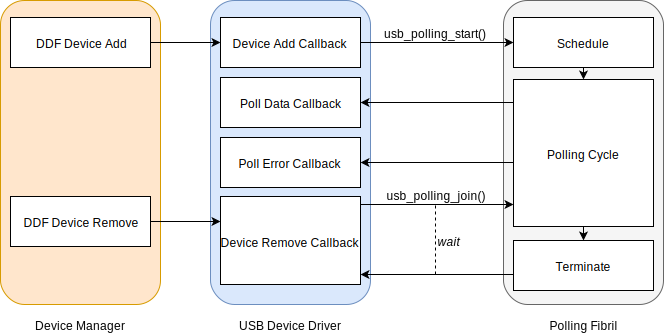
\includegraphics[width=0.8\textwidth]{usb-polling}
	\caption[USB device polling interactions diagram.]{A diagram of interactions
	between the Device Manager, USB device driver and one of its polling fibrils
	during its lifecycle.}
	\label{fig:usb-polling}
\end{figure}

The configuration structure \struct{usb_device_auto_polling_t} has been renamed
for simplicity sake to \struct{usb_polling_t}. Instead of serving as a one-time
configuration structure during polling initiation, its role changed to represent
the entire instance of the polling process throughout its lifetime.

Introducing standard functions such as \fnc{usb_polling_init()} and
\fnc{usb_polling_fini()}, the device driver is now fully responsible for the
ownership of the structure. This is convenient, since drivers often have their
own structures for device data, where \struct{usb_polling_t} can be placed as a
field, dropping the need for additional calls to \fnc{malloc()} and
\fnc{free()}. In addition, this resolves the problem with default values of
various configuration parameters, since in \fnc{usb_polling_init()} all
parameters are assigned their default values and device driver can override only
those desired.

All four of the original polling initialization functions were unified into a
single function \fnc{usb_polling_start()}. Since there is now a clear structure,
which represents the polling instance, the arguments of the original four
functions were moved to \struct{usb_polling_t}, where they are clearly named and
documented, preventing any possible errors from their misinterpretation. Suffice
it to say, that the original four functions mostly fulfilled the role of syntax
sugar, which is now rendered unnecessary, given the fact that default values of
configuration parameters are pre-filled in the polling structure.

Lastly, the API was extended with the \fnc{usb_polling_join()} function, which
closes the polling pipe and consistently waits until the polling fibril
terminates. This function addresses the problem of spinning in driver's
\fnc{device_remove()} or \fnc{device_gone()} callbacks, or possible negligence,
which may result in the polling fibril outliving the device and then accessing
invalid memory. Calling this function in this context will result in the
immediate and synchronous termination of the polling mechanism prior to
deallocation (as depicted in Figure \ref{fig:usb-polling}).

Furthermore, the exposure of internal polling parameters now gives device
drivers more creativity in their approach to polling. For instance, drivers can
now inquire about the state of the polling fibril without the need to have a
private flag maintained by their polling callbacks. The drivers can also change
polling parameters such as request size or polling delay mid-flight, which is a
more flexible approach than to stop polling, change parameters and then start
polling again (note that stopping polling at will was not supported by the
previous implementation without generating actual errors from the hardware
device).

A nice minimalist example of the new polling mechanism usage can be found in
Listing \ref{lst:polling-example}

\begin{listing}
	\begin{code}
		static usb_polling_t polling;
		static uint8_t buffer[13];

		static bool callback(usb_device_t *dev, uint8_t *buffer, size_t size, void *arg)
		{
			printf("Have data!/n");

			// Return true if we wish to continue polling.
			return true;
		}

		static void demo()
		{
			// Initialize.
			usb_polling_init(&polling);

			// Configure.
			polling.device = /* some usb_device_t here */;
			polling.ep_mapping = /* some interrupt(in) endpoint of the device */;
			polling.buffer = buffer;
			polling.request_size = sizeof(buffer);
			polling.on_data = callback;

			// Start polling.
			usb_polling_start(&polling);

			// Sleep synchronously for a while.
			async_usleep(10000);

			// End polling and clean up.
			usb_polling_join(&polling);
			usb_polling_fini(&polling);
		}
	\end{code}
	\caption{Minimal usage example of the new USB device polling mechanism.}
	\label{lst:polling-example}
\end{listing}



\section{USB hub port refactoring - title pending}
\label{hub-port-refactoring}

% TODO @aearsis: Explain the complexity of the topic and the proper solution


\section{A driver for USB tablet}

This modification is very standalone and seemingly simple, yet very useful and
appreciated. We extended the HID driver to support absolutely positioned
devices. That means, one can now connect a USB tablet and it will work in
HelenOS. If you are still wondering what this could be useful for (people using
USB tablets are usually graphic designers or photographers, not microkernel
developers), try running QEMU with an emulated one:

\begin{bdsh}
$ qemu-system-x86_64 -enable-kvm -usb -device usb-tablet -boot d -cdrom image.iso
\end{bdsh}

When using mouse with relative positioning (PS/2, USB mouse), one has to first
click inside the window of QEMU to let it grab input. To release it again,
a special key combination (for current QEMU Ctrl+Alt+G) must be pressed. When
using an emulated USB tablet instead, the mouse is not ``locked'' inside the
window, but it can freely move in and out and still be registered by the guest
OS.

\chapter{Writing USB Drivers}

This chapter provides documentation and general guidelines for usage of the
refactored USB device driver interface. As such, it is meant for developers of
HelenOS device drivers, who can use it as a reference guide. By intention, this
section abstracts the reader from all modifications to the stack, and focuses
only on the latest state of the interface. All changes to the interface are
described in detail in Chapter \ref{usb-refactoring}.

The reader should note that there exists a similar section in the initial USB
stack documentation. The text in this chapter could be considered an updated
version or extension of that text.


\section{Basics}
This section gives details on the basic structure of USB device drivers, their
role in the system and components they usually interact with.


\subsection{Framework}
USB device drivers use the generic \textit{Device Driver Framework} available in
HelenOS. Because all USB drivers have similar initialization routines, a thin
layer -- specific to USB devices -- was added above the generic one. This layer
mainly serves as a middleware for easy communication with USB host controller
drivers, performing USB specific resource management and enabling device drivers
to initialize endpoint pipes and interact with USB devices. For those reasons,
USB device drivers are recommended to link with \lib{libdrv} and
\lib{libusbdev}, which contain both aforementioned layers respectively.

It is expected that USB device drivers specify in advance not only their
relevant match identifiers, which are used by the Device Manager to pair new
devices with available drivers, but also all endpoints, which shall be present
on the device through a USB driver structure. Later when a new device is found,
a specialized device structure is prepared and pipe abstractions are
initialized.

Device drivers live the same life cycle as any other drivers controlled by the
\textit{Device Manager}. A quick summary follows:
~
\begin{enumerate}
	\item The driver is started at the convenience of the Device Manager if and
	when a compatible device is found. At startup, the driver registers with the
	USB framework, which in turn registers also with the Device Driver
	Framework.

	\item During its lifetime, the driver receives IPC callbacks from the USB
	Framework, informing it about relevant device events. On the basis of these
	events, the driver then communicates with the device and exposes various
	interfaces to other tasks in the system. At this point, the controlled
	device usually becomes visible and useful to the user.

	\item When there is no more need for the driver to run (i.e. no devices to
	control), the Device Manager terminates the driver to save resources.
\end{enumerate}

In the Device Driver Framework, drivers are the consumers of \textit{devices}
and providers of \textit{functions}. This paradigm allows them to expose an
unlimited number of nodes (representing logical or physical units) for every
device they control. The same basic principle holds for USB drivers as well.


\subsection{Device Callbacks}
As explained in the previous section, USB device drivers are informed about
relevant device events by asynchronous IPC callbacks from the USB framework. To
simplify usage, these callbacks are identical to those of the Device Driver
Framework:
~
\begin{description}
	\item[Add Device] This event notifies the driver that a new device has been
	discovered and matched to it. From this point on, the driver is allowed to
	communicate with the device in order to configure it and expose its
	functions to the rest of the system. Further communication with the device
	will likely depend on remote calls originating from other system tasks
	utilizing the exposed interface.

	\item[Remove Device] This event instructs the driver to immediately disallow
	new user operations on a device, terminate all currently running
	operations in a timely manner, and hand device control back to the system,
	as the device will likely be physically removed from the bus in the
	forseeable future.

	\item[Device Gone] This event informs the driver that a device has been
	physically disconnected from the system without a prior \textit{Remove
	Device} event. Since the device is no longer reachable, the driver is to
	force interrupt all user operations, which were running at the time of
	receiving the event and report failure to the callers.
	
	\item[Offline Function] By receiving this event, the driver is asked by the
	system to explicitly transition a specific function exposed by one of its
	controlled devices into the \textit{Offline} state. The meaning of such
	transition might depend on the interpretation of the function. For more
	information, see the Device Driver Framework Documentation.

	\item[Online Function] By receiving this event, the driver is asked by the
	system to explicitly transition a specific function exposed by one of its
	controlled devices into the \textit{Online} state. Again, the meaning of such
	transition might depend on the interpretation of the function. For more
	information, see the Device Driver Framework Documentation.
\end{description}

The listed events are delivered to device drivers through function calls to
event handlers specified in the main USB driver operations structure (see
Listing \ref{lst:driver-ops-structure} for minimal example). Since there are no
guarantees on the synchronization between calls, the driver is explicitly
responsible for synchronizing accesses to its private data structures as well as
device communication.

\begin{listing}
	\begin{code}
		static int device_add(usb_device_t *dev)
		{
			usb_log_info("Device '%s' added.", usb_device_get_name(dev));
			return EOK;
		}

		static int device_remove(usb_device_t *dev)
		{
			usb_log_info("Device '%s' removed.", usb_device_get_name(dev));
			return EOK;
		}

		static int device_gone(usb_device_t *dev)
		{
			usb_log_info("Device '%s' gone.", usb_device_get_name(dev));
			return EOK;
		}

		static const usb_driver_ops_t driver_ops = {
			.device_add = device_add,
			.device_remove = device_remove,
			.device_gone = device_gone,
		};
	\end{code}
	\caption[Main USB device driver operations structure.]{Main USB device
	driver operations structure with corresponding event handlers. Note that
	events \textit{Offline Function} and \textit{Online Function} do not require
	a handler and can therefore be omitted in the minimal example.}
	\label{lst:driver-ops-structure}
\end{listing}


\section{Device Communication}
% TODO

\subsection{Endpoint Mapping}
% TODO

\subsection{Pipes}
% TODO

\subsection{Automatic Polling}
% TODO


\section{Utilities}
% TODO

\subsection{Logging}
% TODO

\subsection{Descriptors}
% TODO

\subsection{DMA Buffers}
% TODO





% Appendices
\appendix
\chapter{Benchmarks and Testing}

To demonstrate and benchmark performance of the xHCI stack, a proprietary
subsystem has been implemented in HelenOS. The primary function of this
subsystem is to communicate with a custom QEMU USB device over arbitrary
endpoints and provide statistical information related to the communication.
This way, it can be used to verify the correctness of message transmission,
experiment with synchronization and to measure performance indicators.

In addition, since the subsystem is built on top of the USB device driver
framework and has no xHCI-specific requirements, it can be also used to compare
parameters of the xHCI stack with its predecessors.

The subsystem is composed of three parts:
%
\begin{description}
	\item[QEMU fork with proprietary diagnostic device (usb-tmon)]
		This implementation of QEMU contains a virtual USB device, which carries
		the diagnostic device class descriptor.
	\item[USB Diagnostic Device Driver (usbdiag)]
		The usbdiag driver matches with the QEMU diagnostic device and
		facilitates all communication with it. It also exposes a remote
		interface for all HelenOS applications.
	\item[User Frontend Program (tmon)]
		The tmon program is the primary user frontend in shell. It can use the
		interface exposed by usbdiag to perform various tests with diagnostic
		devices and return human-readable results.
\end{description}


\section{QEMU Device}
\label{sec:tmon}

The \texttt{usb-tmon} virtual device is a diagnostic class USB device
created to allow us to test all of the different transfer types on one device,
gather data about the throughput and speed of the communication and validate
the contents of the USB packets sent between HelenOS and a device.

In order to support communications of all types, the device contains an
endpoint for each direction of each transfer type -- i.e. interrupt, bulk and
isochronous. Since we want to both check the speed of the driver and the
correctness of the data sent, each endpoint is duplicated creating two
sets of endpoints -- first set, which does not validate the transferred data,
and a second set, which checks that each four bytes of the data equal to a
predefined macro \macro{CHECK}. Each of these endpoints has an associated
macro that contains its endpoint number which has the form of
\macro{EP_<type>_<direction>} for the first set and
\macro{CHECKED_EP_<type>_<direction>} for the second set, where \texttt{<type>}
can be \texttt{INT} for interrupt transfers, \texttt{BULK} for bulk transfers or
\texttt{ISOC} for isochronous transfers and \texttt{<direction>} can be either
\texttt{IN} or \texttt{OUT}.

\subsection{Monitoring}

Regardless of which of the aforementioned endpoint sets is used, the
\texttt{usb-tmon} device prints information about the transfers it handles
to QEMU's standard output:
%
\begin{description}
	\item[Interrupt]
		Time since last \texttt{IN} or \texttt{OUT} interrupt request in
		microseconds.
	\item[Bulk]
		Amount of bytes transferred in the last second for every second of an
		\texttt{IN} or \texttt{OUT} bulk transfer.
	\item[Isochronous]
		Notification about receiving the request.
\end{description}

\subsection{Implementation}

The implementation of this device is located in the file
\qemufile{hw/usb/dev-tmon.c}{dev-tmon.c} in the helenos-xhci-team/qemu fork of
the official QEMU repository. It contains several key structures and functions:

\begin{description}
	\item[USBTmonState]
		Structure that represents the current state of a \texttt{usb-tmon}
		device.
	\item[desc\_tmon, desc\_device\_tmon, desc\_iface\_tmon]
		These three structures form the descriptor of the device and contain
		information about the device's class, protocol, endpoints etc.
	\item[usb\_tmon\_class\_init]
		Called when QEMU starts, so it is used as a constructor function for the
		virtual device and all relevant data.
	\item[usb\_tmon\_realize]
		Called when an instance of the \texttt{usb-tmon} device gets created and
		is used to initialize a specific instance of \struct{USBTmonState}.
	\item[usb\_tmon\_handle\_attach]
		Called when an instance of the \texttt{usb-tmon} device gets attached to
		the guest OS.
	\item[usb\_tmon\_handle\_control]
		Called when the device receives a control request, in its current
		implementation simply forwards the request to QEMU via
		\fnc{usb_desc_handle_control}.
	\item[usb\_tmon\_handle\_data]
		Called when the device receives an interrupt, a bulk or an isochronous
		data request, determines the receiving endpoint, stores information
		about handled data and if needed, sends or validates a USB packet.
	\item[usb\_tmon\_\{int\textbar bulk\textbar isoc\}\_\{in\textbar out\}]
		Called on specific kinds of transfers and track sent/received data.
\end{description}

These are the structures and functions one needs to modify in order to modify
the behavior of the device. Additionally, the source code contains helper
functions (e.g. time measurement with \fnc{get_now_sec} and \fnc{get_now_usec})
and QEMU debugging/informational functions and structures (e.g.
\struct{desc_strings}, \struct{vmstate_usb_tmon}, \struct{usb_tmon_info} and
\fnc{usb_tmon_register_types}). These should seldom require modification.

For the purposes of modifying or debugging usb-tmon's source code, the header
\qemufile{include/hw/usb.h}{usb.h} contains most of the structure definitions
and function declarations that might be needed.

\subsection{Usage}

To attach an instance of the \texttt{usb-tmon} device to a running QEMU, one
can type \textit{"device\_add usb-tmon"} into QEMU's monitor (which can be
accessed via the Ctrl-Alt-2 key combination or by redirecting the
monitor to QEMU's standard IO by adding \textit{"-monitor stdio"} to QEMU's
startup command). To have QEMU start with \texttt{usb-tmon} attached, they may
add \texttt{"-device usb-tmon"} to their QEMU startup command.


\section{Driver}

% TODO

\section{Frontend}

\subsection{Structure}

The \texttt{tmon} application consists of the following source files:
%
\begin{description}
	\item[\file{uspace/app/tmon/main.c}{main.c}]
		Main entry point, command selection and usage string.
	\item[\file{uspace/app/tmon/commands.h}{commands.h}]
		Executable commands.
	\item[\file{uspace/app/tmon/list.c}{list.c}]
		Implementation of the \textit{"list"} command.
	\item[\file{uspace/app/tmon/tf.h}{tf.h}, \file{uspace/app/tmon/tf.c}{tf.c}]
		Testing framework, common code for all "\fnc{test-*}" commands.
	\item[\file{uspace/app/tmon/resolve.h}{resolve.h},
		  \file{uspace/app/tmon/resolve.c}{resolve.c}]
		Resolving DDF device from string using devman's IPC interface.
	\item[\file{uspace/app/tmon/burst\_tests.c}{burst\_tests.c}]
		Implementation of burst tests.
\end{description}

\subsection{Usage}

\begin{bdsh}
tmon: benchmark USB diagnostic device

Usage: tmon command [device] [options]

      list - Print a list of connected diagnostic devices.
      test-intr-in - Read from interrupt endpoint as fast as possible.
      test-intr-out - Write to interrupt endpoint as fast as possible.
      test-bulk-in - Read from bulk endpoint as fast as possible.
      test-bulk-out - Write to bulk endpoint as fast as possible.
      test-isoch-in - Read from isochronous endpoint as fast as possible.
      test-isoch-out - Write to isochronous endpoint as fast as possible.

      -n --cycles
            Set the number of read/write cycles.
      -s --size
            Set the data size transferred in a single cycle.

If no device is specified, the first device is used provided that it is the
only one connected. Otherwise, the command fails.

\end{bdsh}

\section{Massive Surprise Removal Testing}

As a simple tool to test multiple scenarios regarding device removal, we wrote
a shell script. It helped us find a lot of synchronization issues in hub driver
and HC drivers. The setup is very simple -- just run HelenOS in QEMU with
a management socket located at \mintinline{bash}{$SOCKFILE}:

\begin{bdsh}
$ qemu-system-x86_64 -qmp unix:$SOCKFILE,server,nowait \
	-device nec-usb-xhci -boot d -cdrom image.iso
\end{bdsh}

Then, assuming a QEMU build in a directory \mintinline{bash}{$QEMU_ROOT}, run
the following snippet:

\begin{bdsh}
: ${repeats:=1} ${count:=1} ${driver:=usb-hub}
: ${in_delay:=5} ${out_delay:=$in_delay}

for rep in $(seq 1 $repeats); do
	for i in $(seq 1 $count);do
		echo "device_add driver=$driver id=burst-$i"
	done

	sleep $in_delay

	for i in $(seq 1 $count);do
		echo "device_del id=burst-$i"
	done

	sleep $out_delay
done | python2 "$QEMU_ROOT/scripts/qmp/qmp-shell" "$SOCKFILE" >/dev/null
\end{bdsh}

The first two lines set default values for various parameters. There are
several combinations which we consider interesting.

\subsection{Fast Attach-Detach Test}

In this test, we used a ridiculously big value of \texttt{repeats}, and very
short value of \texttt{in\_delay}, something like a tenth of a second. Running
the script then simulates e.g. a bad cable, which stays connected only for
a short while.

This test does not work correctly with xHCI, because of a bug in QEMU that cannot
be worked around retaining correctness on real HW. QEMU correctly aborts
transfers in a case of device removal, but any transfer scheduled later is just
ignored. That's fine, the xHCI implementation issues a Stop Endpoint command to
force HC release the ring and allow it to deallocate abort the transfer itself.
Except that QEMU for some reason doesn't allow issuing a Stop Endpoint command
for the default control endpoint. So, in case of bad timing, we can issue
a transfer on EP 0 (like reading the device descriptor as a part of
enumeration) after QEMU knows that the device is removed, but we don't know it
yet. After that, we issue a Stop Endpoint command, which fails. Because we
cannot know whether the endpoint is used or not after the command fails, we
cannot simply abort the transfer. And because the disconnection handler fibril
must make sure the enumeration fibril is not stopped, this results in an
infinite waiting for QEMU response.

Note that this scenario simulates a real-world scenario, which does not happen
in virtual environment. So we consider it is acceptable that this test fails
because of QEMU.

Other HC drivers handled this test fairly well, because they do not maintain
a soft state in the hardware, they just poll transfers for completion. Thus
they know when it's safe to abort the transfer manually.

\subsection{Balloon test}

We used a scenario with a large number of \texttt{repeats}, large \texttt{count},
and long enough delays (like 15 seconds). We simulate a lot of devices connecting,
waiting for matters to stabilize, then disconnecting the devices again.

The main aspect this test is testing is resource leakage. When the resource
usage grows still after the first few rounds, something must be wrong. This
way, we found a leaking reference in \lib{libdrv}, which resulted in devices
never being dropped. That means that we were the first ever to actually remove
a device from HelenOS.

Also, we discovered that limits of HelenOS are much bigger than those of QEMU.
First, QEMU allows at maximum 64 slots per xHC to be enabled. Even though there
are 127 valid USB addresses available, you cannot connect more than 64 devices
at once. Even worse, after this limit is reached, QEMU will not report an error
-- it will simply enable a slot that is already enabled, resulting in correctly
failed assertions in our code.

The second controller that is failing under QEMU is OHCI, which has a hard
limit of 32 hops through the periodic queue. Because every hub (and HID device
too) has an interrupt endpoint, it is added to the periodic queue. QEMU makes
OHCI fail with an unrecoverable error after it reaches this limit of hops.
Because of it, you can connect at most 30 devices to OHCI under QEMU.

\subsection{Burst test}

The last parameter combination we tried was a bursting one. Using
\texttt{repeats = 1}, \texttt{count = 60}, and \texttt{in\_delay = out\_delay
= 4}. This combination connects a subtree of 60 hubs, and allows an arbitrary
subtree of them to enumerate. The disconnection comes during the enumeration,
which is a tough test for the hub driver. The more considering that the
disconnection comes for all devices at once.

Running this test started the hub refactoring described in section
\ref{hub-port-refactoring}, because neither the hub driver, nor our roothub at
that time was prepared for such situations, and failed hard multiple times.
Also, using this test we discovered the fundamental problem of flat hierarchy
presented to DDF, which is explained in the section \ref{hub-port-refactoring}
as well.

\section{Automated Removal Testing}

% TODO

\section{Try it yourself}

% FIXME: should this be even a separate appendix?

This section provides a brief crashcourse on how to get our work running.

After cloning our repository, HelenOS should be compiled as usual according to
the official guide. Namely, the following two commands should suffice given
that necessary build dependencies are installed:

\begin{bdsh}
$ ./tools/toolchain.sh amd64
$ make PROFILE=amd64
\end{bdsh}

\subsection{Running in QEMU}

A reasonably recent (version 2.10 or newer) QEMU is required.

The script \texttt{ew.py}, which is the official way to launch QEMU with
correct parameters, has been modified to include both an xHCI controller and a
USB tablet device (as introduced in \ref{sec:usb-tablet-driver}) by default.
Therefore, one should just run:

\begin{bdsh}
$ ./tools/ew.py
\end{bdsh}

After the system starts, the tablet device should function correctly. The log
of the HelenOS xHCI driver can be viewed with

\begin{bdsh}
$ edit /log/xhci
\end{bdsh}

Other related logfiles are \texttt{/log/usbhub}, \texttt{/log/usbhid} and
\texttt{/log/usbmid}.

\subsection{Testing with tmon}

\texttt{usb-tmon} (described in \ref{sec:tmon}) is a custom USB device emulated
by QEMU. \texttt{tmon} allows us to read and write data to and from endpoints
types and provides some diagnostics.

To use \texttt{usb-tmon}, first compile our version of QEMU that contains the
\texttt{usb-tmon} driver:

\begin{bdsh}
$ cd qemu
$ mkdir build; cd build
$ ../configure --target-list=x86_64-softmmu
$ make
\end{bdsh}

Then start HelenOS in your freshly-compiled QEMU:

\begin{bdsh}
$ ./tools/ew.py -qemu_path ../qemu/build/x86_64-softmmu/
\end{bdsh}

Then switch to the QEMU monitor (Ctrl+Alt+2) and enter \texttt{device\_add
usb-tmon}. Then switch back to HelenOS (Ctrl+Alt+1) and enter \texttt{tmon
list} to the console. A new device should appear. Now you can start the test,
for example with:

\begin{bdsh}
$ tmon test-bulk-in
\end{bdsh}

\subsection{Running on real hardware}

Our work has been tested on a desktop with Teratrend $\mu$DP720202 Rev. 1.0
PCIe card and on a ThinkPad x240 laptop with Intel 8 series xHC (PCI ID
8086:9C31).  Regarding peripherials, several noname and branded USB2 and USB3
hubs, mice, keyboards, multi-interface keyboards (with multimedia keys) and
flash drives have been tested.

It is possible to boot \texttt{image.iso} on the target computer, however
booting over the network proved to be much more convenient during development.
For netboot, we used GRUB instead of the more widespread pxelinux, as HelenOS
uses \texttt{multiboot} protocol and pxelinux does not support it.

The following commands can be used to generate a PXE GRUB image:

\begin{bdsh}
$ grub-mkimage --format=i386-pc --output=core.img --prefix="(pxe)" pxe tftp
$ cat /usr/lib/grub/i386-pc/pxeboot.img core.img > grub2pxe
\end{bdsh}

Then \texttt{/usr/lib/grub/i386-pc}, all files from
\texttt{helenos/boot/distroot/boot/} and the following \texttt{grub.cfg} are
placed to the TFTP server root and \texttt{grub2pxe} is booted.

\begin{bdsh}
set timeout=1
insmod multiboot
menuentry "helenos" {
  set root=(pxe)
  multiboot /kernel.bin
  module    /ns /boot/ns
  module    /loader /boot/loader
  module    /init /boot/init
  module    /locsrv /boot/locsrv
  module    /rd /boot/rd
  module    /vfs /boot/vfs
  module    /logger /boot/logger
  module    /ext4fs /boot/ext4fs
  module    /initrd.img /boot/initrd.img
}
\end{bdsh}

\chapter{Notes on Compatibility}

% TODO


\chapter{Future Development}

This chapter outlines features, which were considered as optional extension of
the project but were not realized due to time, complexity or other constraints.

\section{Power Management}

The xHCI specification focuses a lot on power management. Devices have multiple
states with respect to the amount of power used, and even links between devices
do. Of course, to fully utilize these features, there must have been
a system-wide mechanism to declare intentions about power management. We're not
there yet.

There are although a few power switches we could toggle just now. Given the
small number of drivers implemented, we could for example make the USB fallback
driver suspend the device.

We consider power management a topic that needs to be addressed on the
system-level, and as such we didn't pay much attention to it.

\section{Asynchronous I/O}

The aspect we care about though is performance. Even when the primary goal of
this project was to allow users to use USB on machines equipped only with xHC,
the performance benefit of USB 3 is not negligible, and could be well worth it.

Every transfer type of USB focuses on different characteristics of the
transfer. The interrupt pipes strive for the lowest latency possible -- in this
field, the synchronous semantics works wery well. The latency between receiving
the interrupt and delivering it is as fast as an IPC reply to a call.

Considering isochronous endpoints, it's simply not possible to satisfy them
with a synchronous API, so we decided to change the semantics to asynchronous
one. The downside of the current approach is that the HC driver is forced to
copy the data out from the shared buffer, because it's ownership is temporary.
But since the isochronous transfers in xHCI are just a proof-of-concept and
there are no drivers for real devices yet, we decided not to optimize
prematurely.

The bulk transfer type can however be utilized both synchronously and
asynchronously, and both have their pros and cons. Synchronous API is easier to
work with, asynchronous could be a lot more performant though. As there is just
one driver using bulk endpoints, we decided not to complicate matters and stay
with synchronous-only API for bulk pipes.

\section{Isochronous Transfers in UHCI+OHCI+EHCI}

The module we implemented in xHCI can be thought of as a generic scheduling
framework for isochronous transfers. The scheduler behaves like a leaky bucket,
scheduling the transfers to xHC at constant rate while throttling the device
driver. This is the most complicated part of handling isochronous transfers,
and implementing an asynchronous API for drivers is a good opportunity to
generify it for other drivers as well.

Implementing the support for isochronous transfers for older HCs is a bit
harder task, though. Those drivers use special data structures for isochronous
transfers, and require the software to schedule transfers so all time
constraints are satisfied. (The xHC does it in hardware, software is just
responsible for issuing transfers fast enough.) Also, because of a heavily
simplified implementation of periodic scheduling in former HC drivers,
a substantial refactoring is inevitable. That however needs a deeper
understanding of inner workings of individual HCIs.

\chapter{Project Specification and Timeline}

This section contains the original project specification, as it was approved by
the project comitee at Faculty of Mathematics and Physics, Charles University.
The actual project realization timeline is also included.


\section{Project Specification (in Czech)}

\subsection{Základní informace}

\begin{description}
	\item[Jméno projektu] HelenOS USB 3.x Stack
	\item[Zkratka] HelUSB3
	\item[Vedoucí] Martin Děcký \email{decky@d3s.mff.cuni.cz}
	\item[Konzultanti] --
	\item[Anotace]
		Rozšíření podpory sběrnice USB a USB zařízení v mikrojádrovém multiserverovém operačním systému HelenOS o revizi 3.0 (resp. 3.1), sjednocení této podpory s dříve implementovanou funkcionalitou pro USB 1.0, 1.1 a 2.0 a další vylepšení.
\end{description}

\subsection{Motivace}

Podpora sběrnice USB v revizi 1.0 a 1.1, která byla naimplementována v rámci Softwarového
projektu v roce 2011 (HelUSB), výrazně rozšířila praktickou použitelnost operačního systému
HelenOS v souvislosti s periferními zařízeními. Na tuto funkcionalitu bylo později navázáno
podporou USB 2.0. V současné době je poslední specifikovaná revize USB 3.0 (z hlediska
hardwarového transportu potom 3.1) a začínají se objevovat počítače, které implementují pouze tuto
revizi (tedy z pohledu operačního systému nejsou zpětně kompatibilní se staršími revizemi). Proto
je vhodné, aby byl operační systém HelenOS doplněn o nativní podporu pro USB 3.0 (resp. 3.1).
Tento projekt je pochopitelně také vhodnou příležitostí pro provedení sjednocení s předchozími
implementacemi a provedení dalších souvisejících vylepšení.

\subsection{Popis projektu}

Primárním předmětem projektu je rozšířit generický framework pro použití USB sběrnic a
implementaci ovladačů USB zařízení v systému HelenOS o podporu USB revize 3.0 (resp. 3.1), při
zachování plné podpory předchozích revizí 1.0, 1.1 a 2.0. Cílem je, aby bylo možné na běžně
dostupném hardwaru využít nejvyšší možnou revizi USB s přihlédnutím k možnostem daných
periferních zařízení. Součástí projektu je také implementace základního demonstrátoru – ovladače
konkrétního fyzického USB host controlleru a ověření funkcionality konkrétních koncových USB
zařízení.

\begin{itemize}
	\item
		Implementace ovladače pro USB host controller podle normy xHCI.
		\begin{itemize}
			\item Podpora přenosových režimů a rychlostí odpovídajících USB 1.0, 1.1, 2.0 a 3.0.
			\item
				Enumerace zařízení na sběrnici USB 3.0 a spouštění příslušných ovladačů koncových USB zařízení (s využitím existujícího Device Driver Frameworku), jsou-li k dispozici.
				\begin{itemize}
					\item Zachování kompatibility s dříve naimplementovanými ovladači host controllerů podle norem OHCI, UHCI a EHCI.
					\item Ideálně zachování možnosti implementovat ovladače koncových USB zařízení nezávisle na použité variantě host controlleru.
				\end{itemize}
			\item Demonstrátor: Ovladač pro xHCI host controller NEC Renesas uPD720200
		\end{itemize}

	\item
		Implementace explicitního mechanismu odpojování USB zařízení (očekávaného i neočekávaného).
		\begin{itemize}
			\item Podpora přerušení USB komunikace (USB communication abort) na hardwarové úrovni bez zablokování ovladače USB zařízení.
		\end{itemize}

	\item Implementace podpory isochronního režimu komunikace USB zařízení.
	\item Volitelná část zadání: Rozšíření USB frameworku o dosud nepodporované vlastnosti (např. správa napájení), o podporu specifických xHCI host controllerů (např. Intel Sunrise Point-H a/nebo contollery integrované na vývojových deskách či SoC čipech typu BeagleBoard, BeagleBone, Raspberry Pi) či jiná vylepšení (např. implementace nových ovladačů koncových USB zařízení jako je DisplayLink, dokončení implementace správy přenosového pásma a výkonu, odladění ovladačů controllerů na jiných platformách).

\end{itemize}

\subsection{Platforma, technologie}

\begin{itemize}
	\item
	Framework a ovladače budou odladěny v simulátoru QEMU a na běžném fyzickém PC
	(obojí pro platformy x86 a x86-64) vybaveném výše uvedeným USB controllerem a
	případně kombinací již dříve podporovaných USB controllerů s použitím již existujících
	ovladačů koncových USB zařízení.

	\item
	Framework a ovladače budou implementovány takovým způsobem, který nebude
	principielně bránit jejich budoucímu využití na jiných platformách než x86 a x86-64.

	\item
	Framework a ovladače budou implementovány takovým způsobem, aby zachovávaly
	celkovou softwarovou architekturu mikrojádrového multiserverového operačního systemu
	HelenOS a aby nedošlo k omezení již dříve naimplementované a odladěné funkcionality (tj.
	podpora OHCI, UHCI atd.).
\end{itemize}


\subsection{Odhad náročnosti}

Na základě zkušeností z dřívějšího Softwarového projektu HelUSB (implementace podpory OHCI,
UHCI) lze říci, že zadání je řešitelským týmem o 5 – 6 studentech zvládnutelné ve standardní době.
Projekt klade na řešitele především následující nároky, ze kterých přirozeně plyne přibližný
harmonogram prací:

\begin{itemize}
	\item Nastudování specifikace sběrnice USB, specifikace xHCI, specifikace controlleru NEC Renesas uPD720200, volitelně studium implementací v jiných operačních systémech. [1 měsíc]

	\item Nastudování softwarové architektury, relevantních mechanismů a existující implementace systému HelenOS (async framework, Device Driver Framework, podpora OHCI, UHCI, EHCI). [1 měsíc]

	\item Implementace podpory xHCI a controlleru NEC Renesas uPD720200, integrace s existující implementací, refactoring. [2 měsíce]

	\item Implementace explicitního mechanismu odpojování USB zařízení, přerušení USB komunikace a isochronního režimu komunikace. [1,5 měsíce]

	\item Implementace vhodné podmnožiny volitelných částí zadání. [2,5 měsíce]

	\item Důkladné odladění výsledné implementace, sepsání dokumentace. [1 měsíc]
\end{itemize}

Aktuální stav systému HelenOS poskytuje dostatečně stabilní základ pro úspěšnou realizaci
projektu, riziko nedokončení projektu je malé. Zadání projektu záměrně klade důraz na elegantní
integraci výsledného řešení s existujícím kódem včetně nutného refactoringu. Nelze pochopitelně
zcela vyloučit nutnost opravovat drobné chyby v existující implementaci, které mohou být
v průběhu práce na tomto projektu odhaleny, nemělo by se však jednat o zásadní překážky.

Protože časovou náročnost implementace povinných bodů zadání není možné předem zcela
spolehlivě odhadnout, počítá zadání také s volitelnými částmi, které by posloužily jednak pro
zlepšení celkové funkcionality USB v systému HelenOS a jednak umožnily dosáhnout za všech
okolností obvyklého objemu implementačních prací v rámci Softwarového projektu. V případě, že
povinné části zadání zaberou odhadovaný čas, bude možné implementovat vhodnou podmnožinu
volitelných částí. Ukáže-li se naopak, že odhad časové náročnosti povinných částí byl
podhodnocen, resp. nadhodnocen, potom bude možné omezit, resp. rozšířit, podíl implementace
volitelných částí.


\subsection{Vymezení projektu}

Projekt je zaměřen na následující oblasti:
~
\begin{itemize}
	\item softwarové inženýrství,
	\item vývoj software,
	\item systémové programování,
	\item spolehlivé systémy.
\end{itemize}


\section{Project Timeline}

This section contains the full timeline of project realization throughout the
years 2017 and 2018.

\begin{table}[h]
	\centering
	{\renewcommand{\arraystretch}{1.2}
	\begin{tabularx}{0.95\textwidth}{rl}
		\hline \textbf{April 18, 2017} & Project specification finalized. \\
		\hline \textbf{May 1, 2017} & Project officially started. \\
		\hline \textbf{June 8, 2017} & First commit in the project branch. \\
		\hline \textbf{October 17, 2017} & USB mouse driver transmitting
		movement data over the xHCI stack. \\

		% TODO

		\hline \textbf{February 1, 2018} & Project submitted for defense. \\
		\hline
	\end{tabularx}
	}
	\caption{Project timeline.}
	\label{tbl:timeline}
\end{table}



\end{document}

